\documentclass[preprint,12pt,3p]{elsarticle}

\usepackage{amsmath,amssymb,amsfonts,bm}
\usepackage{booktabs}
\usepackage{multirow}
\usepackage{graphicx}
\usepackage{hyperref}
\usepackage{microtype}
\usepackage{xcolor}
\usepackage{tabularx}

\journal{Computer Methods in Applied Mechanics and Engineering}

\begin{document}

\begin{frontmatter}

\title{Defect-Constrained Stateful Maintenance of Two-Level Schwarz Preconditioners for Evolving Sparse Linear Systems}

\author[inst1]{JSR Research Group\corref{cor1}}
\ead{jsr-research@domain.org}
\cortext[cor1]{Corresponding author}

\affiliation[inst1]{organization={Computational Mathematics and High-Performance Engineering Laboratory},
            addressline={Science and Technology Campus}, 
            city={Metropolis},
            postcode={100000}, 
            country={Country}}

\begin{abstract}
Sequences of evolving sparse SPD operators arise in computational mechanics and make persistent Schwarz factors progressively stale. We propose defect-constrained joint stateful repair (DC-JSR), a maintenance policy based on an accumulated normalized diagonal-variation proxy. With one prescribed tolerance, the unique minimum-cardinality refresh set is the set of blocks whose accumulated proxy exceeds that tolerance. The current Galerkin coarse operator is updated at each step within a fixed two-level symmetric additive Schwarz architecture. A diagonal endpoint bound includes the necessary intermediate-to-current norm ratios; the proxy is not asserted to bound spectral perturbations. On three 3-D FEM operator trajectories, four cyclically ordered single-process timing repetitions give mean DC/Full maintenance-and-certified-solve time ratios of 0.847, 0.977, and 0.929; a fourth trajectory, repeated twice, gives 0.932. Fixed K=3 reaches 245 and 201 PCG iterations in multi-front and compound sequences, whereas DC-JSR reaches 54 and 61, respectively. All 876 audited solves satisfy independent relative true residuals below $10^{-8}$, with a maximum of $3.276221\times10^{-9}$. Additional single-node MPI tests with eight fixed subdomains and one, two, or four processes retain gentle-sequence savings, while multi-front measurements include near-parity and negative configurations. The results quantify maintenance savings, iteration penalties, and the distinction between reduced work and reduced parallel wall time.
\end{abstract}

\begin{keyword}
Domain decomposition \sep Two-level Schwarz preconditioner \sep Symmetric Weighted Additive Schwarz \sep Sparse direct solver \sep MUMPS \sep Evolving linear systems \sep Stateful preconditioner maintenance
\end{keyword}

\end{frontmatter}

\section{Introduction}
\label{sec:intro}

\subsection{Evolving Discrete Operators and Persistent Local Factors}
Computational mechanics problems with changing coefficients, moving sources,
or evolving localized material response give rise to sequences of sparse
linear systems. We consider the SPD case
\begin{equation}
A_t x_t=b_t,\qquad t=0,\ldots,T,
\label{eq:seq_linear_systems}
\end{equation}
with a fixed set of degrees of freedom and a fixed overlapping partition.
Thermal transport and localized damage provide motivating settings
\cite{michaleris2014modeling,lemaitre2005engineering}. Our object of study is
the maintenance of the algebraic preconditioner along a prescribed operator
sequence. Moving-Gaussian-source FEM matrices supply the discrete testbed;
the contribution concerns factor reuse and certified linear solves.

Two-level overlapping Schwarz methods combine local corrections with a
global coarse correction \cite{toselli2005domain,doval2008domain,smith1996domain}.
Sparse direct solvers make the local corrections reliable, but repeated
factorization can be expensive \cite{amestoy2001fully,li2005overview}.
Rebuilding every local factor tracks the current operator; retaining old
factors saves maintenance work but introduces operator mismatch. The relevant
decision is therefore which cached local factors to replace at each step.

\subsection{Why a Single-Step Change Is Not a Reuse State}
A single-step indicator measures the change from $A_{t-1}$ to $A_t$.
A cached factor, however, represents $A_i(\tau_i)$, where $\tau_i$ is its last
refresh step. Several individually small changes can accumulate during this
reuse interval, even when no individual increment exceeds an instantaneous
threshold. Conversely, a sudden relocation or simultaneous activation of
several fronts can require many local updates at once. A fixed refresh count
does not express either the accumulated history or the current number of
blocks whose reuse state has changed substantially.

This motivates an explicit variation state attached to each cached factor.
The state accumulates algebraic increments while that factor is reused and
restarts when the factor is refreshed. This identifies the interval over which
reuse is assessed without prescribing a fixed refresh budget or using solver
iteration feedback to decide maintenance.

\subsection{Defect-Constrained Maintenance and Contributions}
The question addressed here is
\begin{equation}
\text{Which local factors must be refreshed as } A_t\text{ evolves?}
\label{eq:central_research_question}
\end{equation}
We formulate defect-constrained joint stateful repair (DC-JSR) using accumulated
normalized diagonal variation. For a prescribed tolerance $\varepsilon$, the
refresh set is precisely the set of blocks whose accumulated proxy exceeds
that tolerance. The budget is the cardinality of this set, rather than a
separate controller input. Zero, partial, and full refresh follow from the
same rule. The fixed coarse basis is retained while its Galerkin operator is
synchronized with the current global matrix.

The contributions are:
\begin{enumerate}
\item A factor-associated algebraic variation state and a single-tolerance
maintenance policy, with a direct solution of the defect-constrained
minimum-cardinality subset problem. The selection is a linear threshold scan,
not a combinatorial optimization algorithm.
\item A precise account of what the state certifies: a diagonal endpoint bound
with intermediate-to-current norm ratios, and a distinction between this
proxy constraint and independent sufficient conditions for spectral stability.
\item A reproducible two-level FEM operator-sequence evaluation with repeated
timing, direct adaptive-controller and fixed-budget comparisons, complete
refresh histories, and independent true-residual certification. The results
quantify maintenance savings together with iteration penalties; a separate
finite single-node MPI study tests whether these savings persist in parallel.
\end{enumerate}
Neither selective factorization nor cumulative triggering is claimed to be
new in isolation. The method is specified by its particular accumulated
algebraic state, reuse-interval reset, residual-proxy constraint, and operation
within a fixed two-level architecture. Its practical value is assessed on
the operator sequences reported below.

\section{Related Work}
\label{sec:related_work}

\subsection{Schwarz Architecture and Reuse of Solver Information}
Overlapping Schwarz and its coarse-space extensions provide the underlying
solver architecture \cite{schwarz1870ueber,dryja1994domain,toselli2005domain}.
Restricted additive Schwarz changes the local prolongation
\cite{cai1999restricted}; our PCG experiments use symmetric weighted additive
Schwarz. The two-level construction is established background, not a new
preconditioner introduced by DC-JSR.

Krylov recycling retains search-subspace information across related solves
\cite{parks2006recycling,kilmer2006recycling}. Selective maintenance instead
changes the cached factors used to apply the preconditioner. These operations
address different reusable objects and can be combined; recycling methods
should not be classified generally as limited to invariant matrices.
Partial-update domain-decomposition strategies also reduce setup work
\cite{berenguer2015asynchronous,carreno2022strategies}. Cyclic and fixed-count
schedules are useful comparison mechanisms, but the schedule itself need not
encode cumulative variation since a particular factor was constructed.

\subsection{Localized Physical Updates and Performance-Guided Maintenance}
Svolos et al.\ \cite{svolos2020updating} divide dynamic-fracture problems into
localized-failure and healthy regions, updating the former and selectively
reusing the latter. Their healthy-region update strategy uses an idealized
performance optimization based on measured execution time. This is a
physics-assisted, performance-guided maintenance method, not simply a
memoryless damage threshold. DC-JSR instead uses a per-block algebraic
variation state and a prescribed proxy tolerance within a two-level solver.
This distinction does not imply that the earlier method cannot be adapted
to another application.

\subsection{Representative Trigger Mechanisms and the DC-JSR Distinction}
Table~\ref{tab:differentiation} separates state information, trigger logic, and
coarse treatment. The instantaneous and reactive columns describe explicit
representative mechanisms, not universal properties of all algebraic or
lagged-update methods. In particular, algebraic matrix access does not itself
require a physical-field sensor, and a single-step trigger can be used with
either a one-level or a two-level preconditioner.

\begin{table}[htbp]
\centering
\scriptsize
\caption{Representative maintenance mechanisms. Trigger choice and
preconditioner architecture are distinguished. The Svolos column describes
the reported formulation; the instantaneous and reactive columns are
conceptual comparators, not claims about entire method families.}
\label{tab:differentiation}
\begin{tabularx}{\linewidth}{@{}p{0.14\linewidth}XXXX@{}}
\toprule
Dimension & Instantaneous drift trigger & Svolos et al.\ (2020)
& Reactive solver trigger & \textbf{DC-JSR (this work)} \\
\midrule
Decision information
& Current single-step matrix change
& Physical localization and measured execution time
& Iteration, residual, or timing history
& Accumulated diagonal variation since local refresh \\
Physical-field input
& Not required for an algebraic trigger
& Application-specific localization
& Not required for a solver-history trigger
& Not required; assembled matrix and partition are given \\
Coarse treatment
& Independent architecture choice
& Reported single-level ASM
& Independent architecture choice
& Fixed two-level basis; current $Z^TA_tZ$ at every step \\
Refresh rule
& Per-step threshold or ranked fixed-count selection
& Localized-region updates and selective healthy-region reuse
& Update after the specified solver signal
& $S_t^\star=\{i:V_i^-(t)>\varepsilon\}$ \\
Reuse-interval memory
& Absent in a single-step-only trigger
& Physical classification and performance history
& Solver history, rather than prior diagonal path variation
& State accumulates while skipped and resets on refresh \\
Characteristic boundary
& Subthreshold increments may accumulate unnoticed
& Localization must be specified for the application
& Solver work is expended before a post-solve trigger
& Refresh occurs upon proxy crossing; diagonal changes do not capture all matrix changes \\
\bottomrule
\end{tabularx}
\end{table}

The contribution is the explicitly defined factor-associated state and
single-tolerance policy, rather than the mere combination of a threshold and
a coarse solve. Accumulated variation is a policy-level condition for reuse;
it is not a certificate that an inverse remains spectrally accurate.
The closest alternatives must therefore be distinguished by the measured
quantity, its temporal reference, its reset event, and the update rule.

The experimental physics-aware selectors are labeled Svolos-inspired
adaptations, not reproductions of the original fracture algorithm. Likewise,
the directly tested AB-JSR controller remains a separate comparator.
Section~\ref{sec:method} specifies the current DC-JSR policy;
Section~\ref{sec:results} contains its confirmed results. Earlier selectors and
their unchanged numerical tables are recorded separately in
Appendix~\ref{sec:evolutionary_baselines}.

\section{Method: Defect-Constrained Stateful Schwarz Maintenance}
\label{sec:method}

\subsection{Operator Sequence and Two-Level Architecture}
We consider a prescribed sequence of sparse symmetric positive definite (SPD)
systems $A_t x_t=b_t$, $t=0,\ldots,T$. The maintenance problem concerns the
discrete operators and their cached local factors; it does not require a
particular constitutive model or a coupled multiphysics time integrator.
Localized changes motivate selective maintenance, but the policy also permits
simultaneous changes in all subdomains.

Let $R_i$ restrict to overlapping subdomain $i$, and let $D_i$ be positive
diagonal partition-of-unity weights, with
$\sum_i R_i^T D_i R_i=I$. Define $A_i(t)=R_i A_t R_i^T$.
For a fixed, full-column-rank coarse basis $Z$, set
\begin{equation}
A_0(t)=Z^T A_t Z.
\label{eq:dc_coarse_operator}
\end{equation}
The fully refreshed symmetric two-level additive Schwarz preconditioner is
\begin{equation}
P_t=\sum_{i=1}^M R_i^T D_i A_i(t)^{-1}D_i R_i
       +Z A_0(t)^{-1}Z^T.
\label{eq:two_level_prec}
\end{equation}
In the maintained preconditioner, $A_i(t)^{-1}$ is replaced by the inverse
associated with the latest successful local refresh at step $\tau_i$.
Symmetric restriction and prolongation preserve compatibility with PCG.
The audited experiments use continuous piecewise-linear FEM on
$\mathrm{UnitCubeMesh}(N,N,N)$, with $(N+1)^3$ degrees of freedom;
the maintenance construction itself also applies to other SPD discretizations.

\subsection{Persistent Algebraic Variation State}
\label{subsec:diag_proxy}
Write $\mathbf d_i(t)=\operatorname{diag}(A_i(t))$ and define the
dimensionless local increment
\begin{equation}
v_i(t)=\frac{\|\mathbf d_i(t)-\mathbf d_i(t-1)\|_2}
                  {\|\mathbf d_i(t)\|_2}.
\label{eq:dc_increment}
\end{equation}
The denominator is nonzero for SPD local matrices. Initially all local factors
are built from $A_{t=0}$, and $V_i(0)=0$. Before the decision at step $t$, accumulate
\begin{equation}
V_i^-(t)=V_i(t-1)+v_i(t).
\label{eq:dc_state_evolution}
\end{equation}
The preconditioner state consists of the persistent local solver contexts,
their build steps, the current coarse operator, and one decision scalar per block:
\begin{equation}
\mathcal M_t=\bigl(\{K_i\}_{i=1}^M,\{\tau_i\}_{i=1}^M,
                        A_0(t),\{V_i(t)\}_{i=1}^M\bigr).
\label{eq:state_tuple}
\end{equation}
Here $V_i$ is an \emph{algebraic stale-state proxy}, specifically an accumulated
normalized diagonal variation. It is not a spectral-error estimator.
The build step records factor provenance; it does not enter a separate
priority weighting or trigger rule.

\subsection{Defect-Constrained Minimum-Cardinality Subset Selection}
For a refresh set $S$, define the residual proxy
\begin{equation}
R_t(S)=\max_{i\notin S}V_i^-(t),\qquad \max\emptyset:=0.
\label{eq:dc_residual_proxy}
\end{equation}
With prescribed maintenance tolerance $\varepsilon\ge0$, equal local costs give
\begin{equation}
S_t^\star\in\arg\min_{S\subseteq\{1,\ldots,M\}}|S|
\quad\text{subject to}\quad R_t(S)\le\varepsilon.
\label{eq:dc_subset_problem}
\end{equation}
\noindent\textbf{Proposition (Closed-form optimal refresh set).}
The unique solution of \eqref{eq:dc_subset_problem} is
\begin{equation}
\boxed{S_t^\star=\{i:V_i^-(t)>\varepsilon\}.}
\label{eq:dc_closed_form}
\end{equation}
It also uniquely minimizes $\sum_{i\in S}c_i$ for any strictly positive costs
$c_i$. Indeed, every feasible set must contain every block whose proxy exceeds
$\varepsilon$. The set in \eqref{eq:dc_closed_form} is feasible, and adding any
other block strictly increases the cost. \hfill $\blacksquare$

Refactorize precisely the selected blocks. After successful refresh, commit
\begin{equation}
V_i(t)=\begin{cases}0,&i\in S_t^\star,\\
V_i^-(t),&i\notin S_t^\star,\end{cases}
\qquad
\tau_i\leftarrow t\quad(i\in S_t^\star).
\label{eq:dc_state_commit}
\end{equation}
Consequently $\max_i V_i(t)\le\varepsilon$.
The budget $K_t=|S_t^\star|$ is an output of the constraint: zero refresh,
partial refresh, and full refresh all follow from the same rule.
During a skipped interval, the state retains each increment. If their
cumulative sum exceeds $\varepsilon$, the block is refreshed at the first
such step, even when every individual increment is subthreshold. This is a
statement about the chosen diagonal proxy, not a guarantee of detecting every
matrix perturbation. A nonzero increment sequence need not have a sum that
crosses the tolerance.

The policy has a single maintenance tolerance. Monitoring costs
$\mathcal O(\sum_i n_i)$ and closed-form selection costs $\mathcal O(M)$.
Sorting, as used in the shadow prototype, is unnecessary for the max constraint.

\subsection{Diagonal Endpoint Bound and Its Limitations}
Let $\tau_i<t$ denote the most recent successful refresh before the current
decision. Along this unrefreshed interval,
\begin{equation}
V_i^-(t)=\sum_{s=\tau_i+1}^{t}
\frac{\|\mathbf d_i(s)-\mathbf d_i(s-1)\|_2}{\|\mathbf d_i(s)\|_2}.
\label{eq:dc_path_sum}
\end{equation}
The triangle inequality gives the normalized diagonal endpoint bound
\begin{align}
\frac{\|\mathbf d_i(t)-\mathbf d_i(\tau_i)\|_2}{\|\mathbf d_i(t)\|_2}
&\le\sum_{s=\tau_i+1}^{t}
\frac{\|\mathbf d_i(s)\|_2}{\|\mathbf d_i(t)\|_2}
\frac{\|\mathbf d_i(s)-\mathbf d_i(s-1)\|_2}{\|\mathbf d_i(s)\|_2}
\notag\\
&\le\gamma_i(t)V_i^-(t),\qquad
\gamma_i(t)=\max_{\tau_i<s\le t}
\frac{\|\mathbf d_i(s)\|_2}{\|\mathbf d_i(t)\|_2}.
\label{eq:dc_endpoint_bound}
\end{align}
The norm-ratio factor cannot generally be dropped. For the scalar positive
diagonal sequence $10\to5\to1$, the path state is $5$, while the current
normalized endpoint drift is $9$. Closed oscillations can also have zero
endpoint drift and positive path state. Thus accumulated variation retains
history and may be conservative under reversals; it does not eliminate all
effects of elapsed reuse. These statements concern diagonal vectors only:
neither \eqref{eq:dc_endpoint_bound} nor $R_t(S)\le\varepsilon$ bounds a
generalized-eigenvalue perturbation or the PCG iteration count.

\subsection{Coarse Synchronization and Positive Definiteness}
The coarse operator \eqref{eq:dc_coarse_operator} is assembled and factored at
every step, including steps with $S_t^\star=\emptyset$. The basis $Z$ is fixed;
this updates the coarse operator, not the coarse basis. With the committed
build steps, the maintained preconditioner is
\begin{equation}
Q_t=\sum_{i=1}^M R_i^T D_i A_i(\tau_i)^{-1}D_i R_i
       +Z A_0(t)^{-1}Z^T.
\label{eq:dc_maintained_preconditioner}
\end{equation}
If the current global operator and cached local operators are SPD, the positive
weights cover all degrees of freedom, and $Z$ has full column rank, then $Q_t$
is SPD: each summand has a nonnegative quadratic form and for every nonzero
vector at least one local summand is strictly positive. This structural
property permits PCG with stale factors; it does not imply a uniform
condition-number bound. Coarse synchronization is a fixed feature of the
two-level architecture, rather than an additional adaptive decision.

\subsection{Theoretical Foundation: Conditional Spectral Stability}
\label{subsec:theory_stability}

For context, the following conditional perturbation proposition compares full and maintained preconditioners under an independently assumed bound on complete local operators. It is not a spectral guarantee of the diagonal-proxy maintenance rule.

Let $A_t \in \mathbb{R}^{n \times n}$ be an SPD operator at step $t$. Let $P = M_{\text{exact}}^{-1}(A_t)$ denote the exact two-level Symmetric Weighted Additive Schwarz preconditioner defined in \eqref{eq:two_level_prec}, and let $Q = M_t^{-1}$ denote a statefully maintained preconditioner where a subset $\mathcal{S}_t \subset \{1, \dots, M\}$ is refactorized using current local operators $A_i(t)$, while unrefactored subdomains $j \notin \mathcal{S}_t$ retain historical direct factors $A_j(\tau_j)$ with $\tau_j < t$, and the Galerkin coarse operator $A_0(t) = Z^T A_t Z$ is synchronized:
\begin{equation}
Q = \sum_{i \in \mathcal{S}_t} R_i^T D_i A_i(t)^{-1} D_i R_i + \sum_{j \notin \mathcal{S}_t} R_j^T D_j A_j(\tau_j)^{-1} D_j R_j + Z A_0(t)^{-1} Z^T.
\label{eq:stateful_prec_decomp}
\end{equation}

\noindentThe spectral assumption below uses a separate parameter $\eta$; it is not implied by the DC-JSR maintenance tolerance $\varepsilon$ or by its diagonal proxy constraint.

\noindent\textbf{Proposition (Conditional Spectral Stability under Bounded Local Drift).}
\textit{Assume that for all unrefactored subdomains $j \notin \mathcal{S}_t$, the symmetric relative operator drift satisfies the spectral-norm bound:
\begin{equation}
\|E_j\|_2 := \left\| A_j(t)^{-1/2} \left( A_j(t) - A_j(\tau_j) \right) A_j(t)^{-1/2} \right\|_2 \le \eta < \frac{1}{2}.
\label{eq:prop_condition}
\end{equation}
Define the relative drift expansion constant $\delta = \frac{\eta}{1 - \eta} < 1$. Then the stateful preconditioner $Q$ satisfies the two-sided quadratic form perturbation bound:
\begin{equation}
(1 - \delta) P \preceq Q \preceq (1 + \delta) P.
\label{eq:quadratic_bound}
\end{equation}
Consequently, the generalized eigenvalues $\lambda_k(Q A_t)$ satisfy:
\begin{equation}
(1 - \delta) \lambda_k(P A_t) \le \lambda_k(Q A_t) \le (1 + \delta) \lambda_k(P A_t) \quad (\forall k=1, \dots, n).
\end{equation}
Because $Q A_t$ is similar to the symmetric positive definite operator $A_t^{1/2} Q A_t^{1/2}$ (and $Q^{1/2} A_t Q^{1/2}$), its spectrum is real and positive. The effective spectral condition number governing Preconditioned Conjugate Gradient (PCG) convergence, defined as $\kappa_{\text{PCG}}(Q A_t) := \lambda_{\max}(Q A_t) / \lambda_{\min}(Q A_t) = \kappa_{\text{sp}}(Q^{1/2} A_t Q^{1/2})$, satisfies:
\begin{equation}
\kappa_{\text{PCG}}(Q A_t) \le \left( \frac{1 + \delta}{1 - \delta} \right) \kappa_{\text{PCG}}(P A_t) = \left( \frac{1}{1 - 2\eta} \right) \kappa_{\text{PCG}}(P A_t).
\label{eq:condition_number_bound}
\end{equation}}

\noindent\textit{Proof.}
For any unrefactored subdomain $j \notin \mathcal{S}_t$, write $A_j(\tau_j) = A_j(t)^{1/2} (I - E_j) A_j(t)^{1/2}$. By the condition $\|E_j\|_2 \le \eta < 1/2 < 1$, the Neumann series expansion yields:
\begin{equation}
A_j(\tau_j)^{-1} - A_j(t)^{-1} = A_j(t)^{-1/2} \left[ (I - E_j)^{-1} - I \right] A_j(t)^{-1/2}.
\end{equation}
Using $\|(I - E_j)^{-1} - I\|_2 \le \|E_j\|_2 / (1 - \|E_j\|_2) \le \eta / (1 - \eta) = \delta$, the local quadratic form satisfies:
\begin{equation}
-\delta A_j(t)^{-1} \preceq A_j(\tau_j)^{-1} - A_j(t)^{-1} \preceq \delta A_j(t)^{-1}.
\end{equation}
Applying the symmetric restriction/weighting operator $R_j^T D_j (\cdot) D_j R_j$ and summing over all skipped subdomains $j \notin \mathcal{S}_t$:
\begin{equation}
Q - P = \sum_{j \notin \mathcal{S}_t} R_j^T D_j \left( A_j(\tau_j)^{-1} - A_j(t)^{-1} \right) D_j R_j.
\end{equation}
Because the diagonal partition-of-unity weights $D_i$ are non-negative, each term $R_i^T D_i A_i(t)^{-1} D_i R_i$ is positive semi-definite (PSD). Summing over the subset $j \notin \mathcal{S}_t$ is bounded by the sum over all subdomains:
\begin{equation}
\sum_{j \notin \mathcal{S}_t} R_j^T D_j A_j(t)^{-1} D_j R_j \preceq \sum_{i=1}^M R_i^T D_i A_i(t)^{-1} D_i R_i = P_{\text{loc}} \preceq P.
\end{equation}
Therefore, $-\delta P \preceq -\delta P_{\text{loc}} \preceq Q - P \preceq \delta P_{\text{loc}} \preceq \delta P$, establishing \eqref{eq:quadratic_bound}. 

Congruence of \eqref{eq:quadratic_bound} by $A_t^{1/2}$ yields the corresponding Loewner bounds between $A_t^{1/2}QA_t^{1/2}$ and $A_t^{1/2}PA_t^{1/2}$. Applying the Courant--Fischer min-max theorem to the symmetric operator $A_t^{1/2} Q A_t^{1/2}$ relative to $A_t^{1/2} P A_t^{1/2}$ yields $(1 - \delta) \lambda_k(P A_t) \le \lambda_k(Q A_t) \le (1 + \delta) \lambda_k(P A_t)$ for all $k$. Taking the ratio $\lambda_{\max} / \lambda_{\min}$ establishes \eqref{eq:condition_number_bound}. \hfill $\blacksquare$


This proposition is an independent sufficient condition on full local matrices. DC-JSR does not evaluate $E_j$, certify $\eta$, or infer this condition from $V_i$.

\subsection{Operator-Family Generalization and Architectural Requirements: 3-D Damaged Linear Elasticity}
\label{subsec:elasticity_generalization}

To establish the mathematical formulation and architectural design requirements for extending stateful selective maintenance beyond scalar diffusion to vector continuum mechanics, consider the 3-D balance of linear momentum for an elastic body undergoing localized progressive damage or phase softening:
\begin{equation}
-\nabla \cdot \boldsymbol{\sigma}(\boldsymbol{u}, t) = \boldsymbol{f}(x), \quad x \in \Omega = (0, 1)^3,
\label{eq:elasticity_momentum}
\end{equation}
where $\boldsymbol{u} = (u_1, u_2, u_3)^T$ is the displacement vector field, and $\boldsymbol{\sigma}$ is the Cauchy stress tensor governed by a time-evolving fourth-order elasticity tensor $\mathbf{C}(x, t)$:
\begin{equation}
\boldsymbol{\sigma}(\boldsymbol{u}, t) = \mathbf{C}(x, t) : \boldsymbol{\varepsilon}(\boldsymbol{u}), \quad \boldsymbol{\varepsilon}(\boldsymbol{u}) = \frac{1}{2} \left( \nabla \boldsymbol{u} + (\nabla \boldsymbol{u})^T \right).
\end{equation}
To ensure positive-definiteness throughout time evolution, we assume uniform strong ellipticity: there exist constants $0 < \alpha_C \le \beta_C < \infty$ such that:
\begin{equation}
\alpha_C \|\boldsymbol{\xi}\|^2 \le \boldsymbol{\xi} : \mathbf{C}(x, t) : \boldsymbol{\xi} \le \beta_C \|\boldsymbol{\xi}\|^2, \quad \forall \boldsymbol{\xi} \in \mathbb{R}_{\text{sym}}^{3 \times 3}, \ \forall x \in \Omega, \ \forall t \ge 0.
\label{eq:strong_ellipticity}
\end{equation}
In localized damage mechanics, this is modeled via $\mathbf{C}(x, t) = (1 - d(x, t)) \mathbf{C}_0(x) + d(x, t) \mathbf{C}_{\text{residual}}$ with damage variable $d(x, t) \in [0, 1)$ and $\mathbf{C}_{\text{residual}} \succ 0$.

Discretizing \eqref{eq:elasticity_momentum} via finite elements or finite differences yields the $3 \times 3$ block sparse system $A_t \boldsymbol{u}_t = \boldsymbol{b}_t \in \mathbb{R}^{3n \times 3n}$. Extending the stateful maintenance framework to this vector operator family introduces two key architectural requirements:
\begin{enumerate}
    \item \textbf{Block-Diagonal Operator-Drift Proxy}: For $3 \times 3$ nodal blocks, scalar diagonal traces can fail to capture off-diagonal shear coupling. We therefore define the block-diagonal Frobenius drift surrogate:
    \begin{equation}
    d_i^{\text{block}}(t) = \sqrt{\sum_{p \in \Omega_i} \left\| A_{t, pp} - A_{t-1, pp} \right\|_F^2},
    \label{eq:block_proxy}
    \end{equation}
    where $A_{t, pp} \in \mathbb{R}^{3 \times 3}$ is the diagonal nodal block at spatial grid point $p$. Evaluating \eqref{eq:block_proxy} retains $\mathcal{O}(n_i)$ computational complexity while capturing the full tensor Frobenius norm of nodal stiffness variations. We emphasize that $d_i^{\text{block}}$ serves as an empirical drift surrogate rather than a certified norm-equivalent estimator of the global operator perturbation.
    \item \textbf{Vector Coarse Space Construction}: Unlike scalar problems where piecewise constant indicators suffice, vector elasticity requires coarse interpolation operators $Z \in \mathbb{R}^{3n \times 3M}$ that span rigid body modes (translations and infinitesimal rotations) or block-component partition indicators ($Z = Z_{\text{scalar}} \otimes I_3$) to prevent low-frequency locking.
\end{enumerate}
This subsection records architectural requirements for a possible vector-operator extension. Such an extension is not evaluated in the DC-JSR audit and is not an additional component of the scalar maintenance policy.

\subsection{Certified Solve and Cost Accounting}
Every solve is accepted only if
\begin{equation}
\operatorname{RelRes}(x_t)=\frac{\|b_t-A_t x_t\|_2}{\|b_t\|_2}<10^{-8}.
\label{eq:rel_res}
\end{equation}
The audit uses $\mathrm{rtol}=5\times10^{-11}$ and
$\mathrm{atol}=10^{-14}$, explicit PETSc true-residual evaluation, and an
independent CSR residual calculation. A failed initial certification permits
a tighter solver retry; it does not change $S_t^\star$. No retry was required
in the 876 audited solves. The maximum true relative residual was
$3.276221\times10^{-9}$.
For identically defined timed work, the net saving over Full Rebuild is
\begin{equation}
\Delta T_{\rm net}=\sum_{t=1}^T
\left[T_{\rm setup}^{\rm full}(t)-T_{\rm setup}^{\rm DC}(t)
      +T_{\rm solve,cert}^{\rm full}(t)-T_{\rm solve,cert}^{\rm DC}(t)
      +T_{\rm monitor}^{\rm full}(t)-T_{\rm monitor}^{\rm DC}(t)\right].
\label{eq:cost_model}
\end{equation}
Here setup includes local and coarse maintenance, and solve includes primary
true-residual certification. Assembly, initialization, and additional audit
checks are accounted for separately. The constraint minimizes required local
refreshes for the chosen proxy; it does not minimize total runtime a priori.

\section{Experimental Results}
\label{sec:results}

\subsection{Primary DC-JSR Audit: Repeated Timing and Certified Solves}
\label{subsec:dc_primary_audit}
The primary single-process evaluation concerns algebraic maintenance on identical prescribed
3-D FEM operator and right-hand-side sequences. Each mesh has $N=24$ intervals
per axis, $15,625$ nodal degrees of freedom and eight overlapping subdomains.
DC-JSR uses the frozen value $\varepsilon=0.08$. Full Rebuild, instantaneous
relative-diagonal-drift Fixed K=3, and the existing AB-JSR controller use the
same local solver and current coarse operator. Four repetitions cyclically
rotate the four methods, placing each method once in every execution position.
The staccato sequence has two position-swapped Full/DC repetitions.
These are repeated and additional-trajectory evaluations, not independently
preregistered blind tests.

\begin{table}[htbp]
\centering
\scriptsize
\caption{Primary DC-JSR timing audit. Times are means $\pm$ sample standard
 deviations in seconds. Ratios are ratios of mean DC and Full times; wins
 compare paired repetitions. The staccato row has two repeats and no AB or
 Fixed K=3 run.}
\label{tab:dc_primary_performance}
\resizebox{\linewidth}{!}{%
\begin{tabular}{lccccccc}
\toprule
Trajectory & Repeats & Full (s) & Fixed K=3 (s) & DC-JSR (s) & AB-JSR (s) & DC/Full & DC wins \\
\midrule
Gentle & 4 & $6.077\pm0.061$ & $5.303\pm0.030$ & $5.146\pm0.028$ & $5.387\pm0.039$ & $0.847$ & 4/4 \\
Multi-front & 4 & $10.541\pm0.143$ & $27.507\pm0.218$ & $10.298\pm0.160$ & $10.541\pm0.094$ & $0.977$ & 3/4 \\
Compound & 4 & $12.054\pm0.142$ & $25.222\pm0.070$ & $11.195\pm0.108$ & $11.443\pm0.086$ & $0.929$ & 4/4 \\
Staccato & 2 & $10.296\pm0.041$ & -- & $9.596\pm0.140$ & -- & $0.932$ & 2/2 \\
\bottomrule
\end{tabular}}
\end{table}

\begin{table}[htbp]
\centering
\small
\caption{Maximum PCG iterations in the primary audit. Equal maxima do not
 imply equal stepwise iteration histories.}
\label{tab:dc_primary_iterations}
\begin{tabular}{lcccc}
\toprule
Trajectory & Full & Fixed K=3 & DC-JSR & AB-JSR \\
\midrule
Gentle & 47 & 47 & 47 & 47 \\
Multi-front & 54 & 245 & 54 & 54 \\
Compound & 53 & 201 & 61 & 53 \\
Staccato & 55 & -- & 55 & -- \\
\bottomrule
\end{tabular}
\end{table}

The timed workload includes monitoring, local and coarse maintenance, CG,
 and primary PETSc true-residual certification; assembly, initialization and
 additional CSR/state/coarse audits are recorded separately. This is a
 maintenance-and-solve comparison on discrete operator sequences generated
 from moving-Gaussian-source FEM matrices.

DC-JSR is faster than AB-JSR in all twelve paired primary repetitions; mean
DC/AB ratios are 0.955, 0.977 and 0.978 for gentle, multi-front and compound
sequences. The multi-front DC/Full ratios are 0.971, 1.004, 0.947 and 0.987:
 the small average benefit does not imply an advantage in every run.
The compound budget is
$[0,4,2,4,4,4,8,2,6,3,7,3,8,2,4,2,4,2]$;
full refresh at steps 7 and 13 follows directly from
\eqref{eq:dc_closed_form}. Compound DC reaches 61 iterations, versus 53 for
Full; savings therefore coexist with an iteration penalty.

\begin{figure}[htbp]
\centering
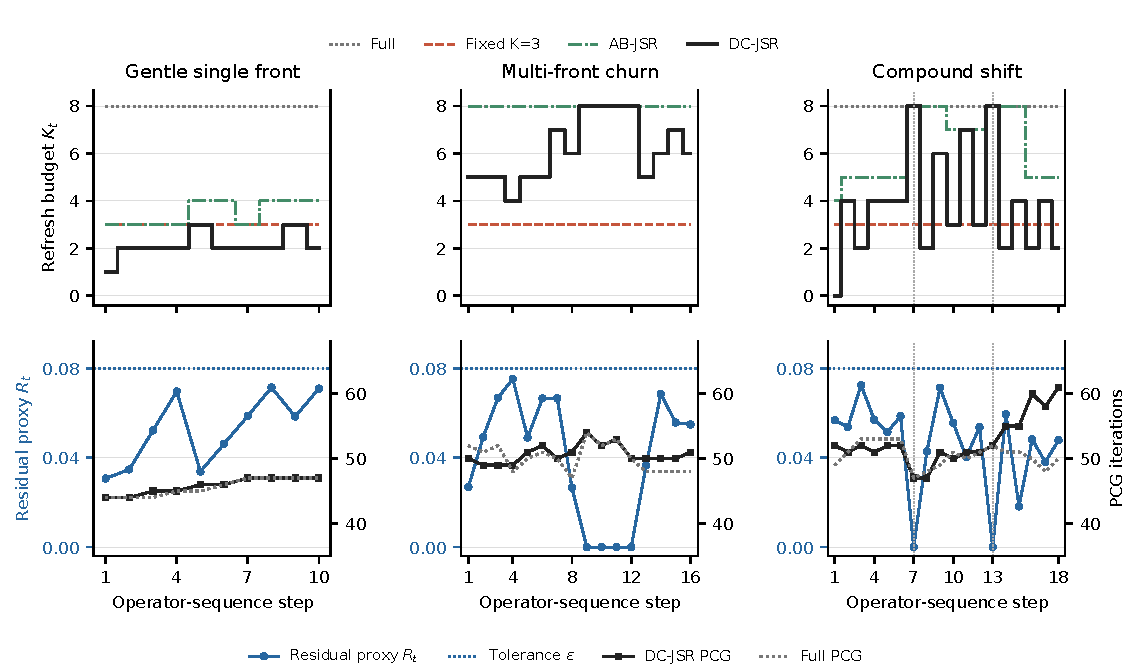
\includegraphics[width=\linewidth]{figures/dc_jsr_budget_proxy_pcg.pdf}
\caption{DC-JSR maintenance on three certified FEM operator sequences.
Top row: refresh budget $K_t$ for DC-JSR and its three comparators.
Bottom row: the post-refresh residual proxy
$R_t(S_t^\star)=\max_i V_i(t)$ (blue, left axis), the tolerance
$\varepsilon=0.08$ (dotted blue), and DC/Full PCG iterations (right axis).
The first repeat is shown; budget and iteration histories are identical
across the four repeats for each method. Vertical guides mark compound
steps 7 and 13. The proxy is not a spectral residual.}
\label{fig:dc_budget_proxy_pcg}
\end{figure}

All 876 audited solves, including the primary repetitions and the separate
compound sensitivity runs at $\varepsilon=0.03,0.05,0.12$, pass both PETSc and
independent CSR true-residual checks; no solver retry is required.
The maximum relative true residual is $3.276221\times10^{-9}$.
The current coarse operator agrees with independently accumulated $Z^TA_tZ$
 to a maximum relative difference of $1.597107\times10^{-13}$.
Two hundred generated eight-block policy instances were checked against all
256 subsets each, including strictly positive unequal maintenance costs.
These finite checks corroborate the closed-form implementation; the general
optimality result is the proposition in Section~\ref{sec:method}.


\subsection{Limited Single-Node MPI Validation}
\label{subsec:dc_mpi_validation}
We additionally evaluate a distributed implementation on the same prescribed
operator family, with $N=24$ and $N=32$ ($15,625$ and $35,937$ degrees of freedom).
The partition remains fixed at eight subdomains as the number of MPI processes
changes through $P=1,2,4$. The single WSL node exposes four logical CPUs of an
Intel Core i5-12490F; each rank is pinned to one logical CPU, with OpenMP and
BLAS thread counts fixed to one. These are finite single-node strong-scaling
measurements, not a multi-node scalability claim.

The global AIJ matrices and PCG vectors are distributed by contiguous rows.
Local factor $i$ is owned by rank $i\bmod P$. PETSc vector scatters exchange
overlapping input entries and add the returned local corrections. The
unchanged threshold rule is evaluated locally by each factor owner. The
fixed eight-dimensional Galerkin operator is assembled by an MPI reduction;
its exact LU is replicated, and each application reduces the coarse right-hand
side. All local factors and the coarse operator are fixed during each PCG solve.

Full and DC use the same distributed backend. Each configuration has one full
warmup per method and four paired repetitions with alternating method order.
Process-count order is cyclically rotated across mesh/workload configurations;
MPI jobs run sequentially. After a step-start barrier, timed work includes
monitoring, selected local submatrix construction and refactorization, coarse
maintenance, PCG, and primary true-residual certification. The step wall time is
\begin{equation}
T_t^{\rm MPI}=\max_{0\le p<P}T_{t,p},
\label{eq:dc_mpi_walltime}
\end{equation}
and sequence time is its sum. Input generation, distributed operator/overlap-row
staging, and additional independent audits are excluded. Static backend setup
and initial factor/coarse construction are separately measured. The snapshot
inputs were reassembled and verified array by array; the $N=24$ matrix/right-hand
side hashes match the original serial audit. Thus the experiment measures
maintenance and solves of preloaded sequences, rather than a complete physical
application with assembly and data-distribution costs.

\begin{table}[htbp]
\centering
\scriptsize
\caption{Finite MPI validation with eight fixed subdomains and
$\varepsilon=0.08$. Times are means $\pm$ sample standard deviations in seconds
across four paired repeats. DC/Full is a ratio of mean times; the Init column
also includes static setup and initial local/coarse factors. Iteration entries
are the maximum Full/DC counts. All configurations and slower DC repetitions
are retained.}
\label{tab:dc_mpi_performance}
\resizebox{\linewidth}{!}{%
\begin{tabular}{llccccccc}
\toprule
$N$ & Trajectory & $P$ & Full (s) & DC (s) & DC/Full & With Init & DC wins & Max.~iters F/DC \\
\midrule
24 & Gentle & 1 & $4.766\pm0.126$ & $3.922\pm0.113$ & 0.823 & 0.829 & 4/4 & 47/47 \\
24 & Gentle & 2 & $2.807\pm0.086$ & $2.289\pm0.022$ & 0.815 & 0.822 & 4/4 & 47/47 \\
24 & Gentle & 4 & $2.090\pm0.022$ & $1.887\pm0.065$ & 0.903 & 0.904 & 4/4 & 47/47 \\
24 & Multi-front & 1 & $8.767\pm0.319$ & $8.362\pm0.156$ & 0.954 & 0.956 & 4/4 & 54/54 \\
24 & Multi-front & 2 & $4.739\pm0.131$ & $5.003\pm0.735$ & 1.056 & 1.054 & 2/4 & 54/54 \\
24 & Multi-front & 4 & $3.796\pm0.044$ & $3.806\pm0.063$ & 1.003 & 1.001 & 2/4 & 54/54 \\
32 & Gentle & 1 & $13.650\pm0.768$ & $10.115\pm0.581$ & 0.741 & 0.757 & 4/4 & 50/51 \\
32 & Gentle & 2 & $8.409\pm0.426$ & $6.243\pm0.215$ & 0.742 & 0.754 & 4/4 & 49/50 \\
32 & Gentle & 4 & $5.373\pm0.093$ & $4.543\pm0.088$ & 0.845 & 0.851 & 4/4 & 49/50 \\
32 & Multi-front & 1 & $26.585\pm1.043$ & $24.361\pm2.337$ & 0.916 & 0.918 & 3/4 & 58/62 \\
32 & Multi-front & 2 & $14.837\pm0.269$ & $14.273\pm0.580$ & 0.962 & 0.962 & 3/4 & 58/62 \\
32 & Multi-front & 4 & $9.641\pm0.683$ & $9.379\pm0.199$ & 0.973 & 0.972 & 2/4 & 58/62 \\
\bottomrule
\end{tabular}}
\end{table}

\begin{figure}[htbp]
\centering
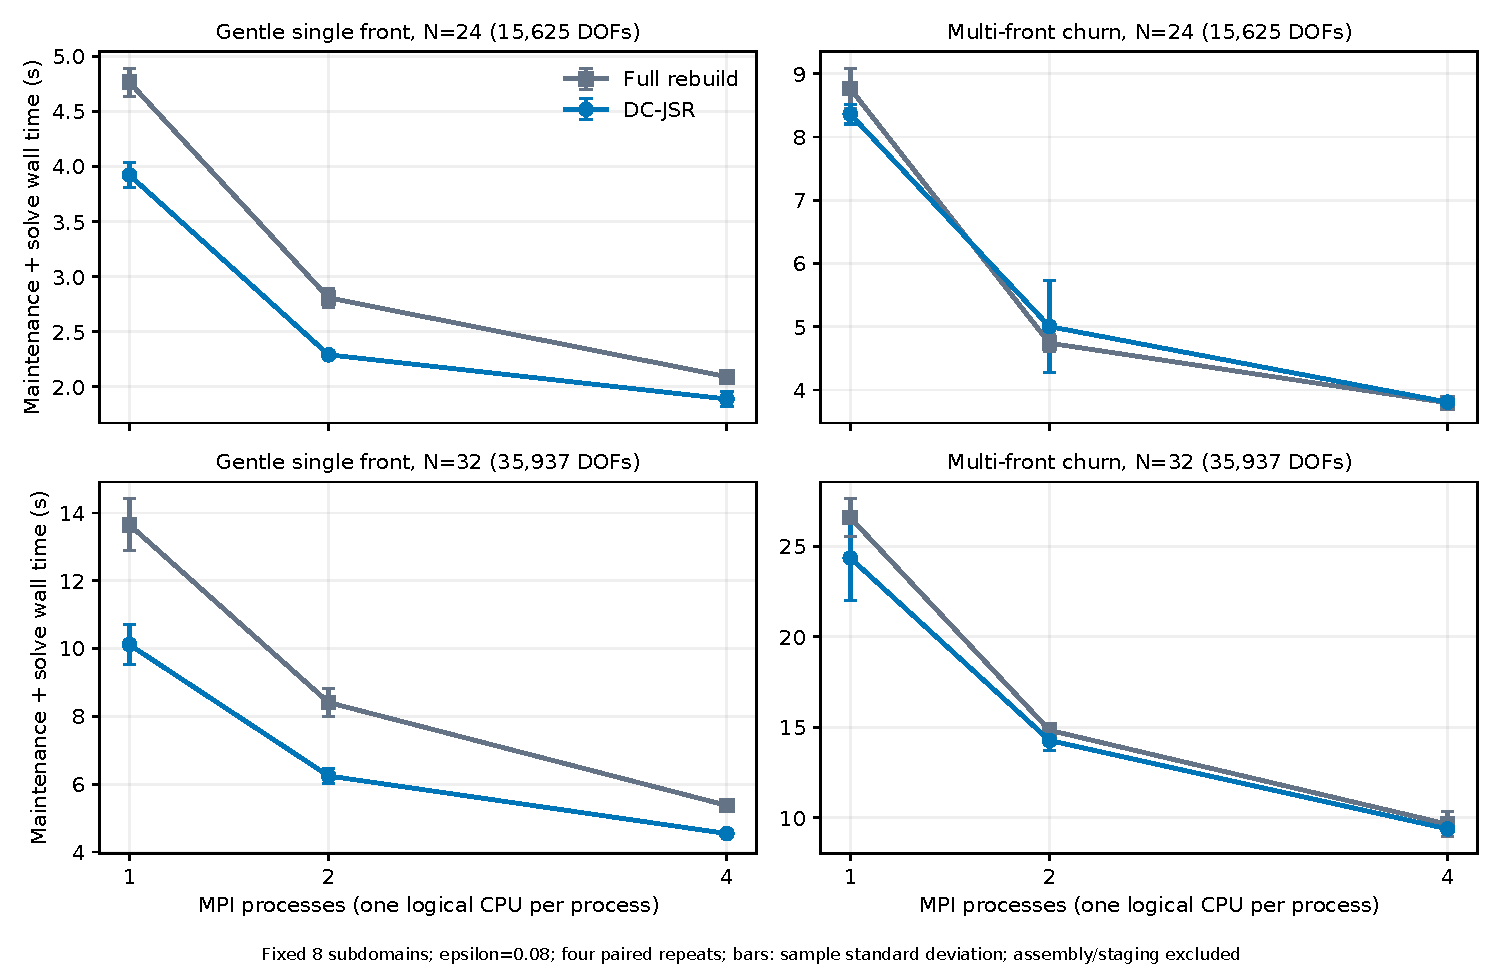
\includegraphics[width=\linewidth]{figures/dc_jsr_parallel_validation.pdf}
\caption{Maintenance-and-certified-solve wall time for $P=1,2,4$ on one
node, with eight fixed subdomains. Error bars are sample standard deviations
of four repetitions. The larger mesh retains gentle-sequence savings, while
multi-front benefits are small and include negative configurations. Assembly,
input staging and initialization are excluded from these curves; initialization
is included in the secondary ratio in Table~\ref{tab:dc_mpi_performance}.}
\label{fig:dc_mpi_validation}
\end{figure}

Gentle-sequence DC/Full ratios at four processes are 0.903 and 0.845 for
$N=24$ and $N=32$, respectively; DC is faster in all 24 gentle paired
comparisons across meshes and process counts. Multi-front four-process ratios
are 1.003 and 0.973, each with only two of four paired wins. The $N=24$
two-process mean ratio is 1.056, with a relatively large DC standard deviation:
one retained DC repeat takes 6.099\,s versus its paired Full time of 4.645\,s.
The data do not identify the source of this execution variability.
On $N=32$ multi-front, DC reaches 62 iterations versus 58 for Full.

The distinction between local work and the parallel critical path is material.
For $N=32$ gentle at four processes, mean accumulated rank-local maintenance
work decreases from 6.431 to 1.543\,s, whereas the sum of stepwise maximum-rank
local times decreases from 1.672 to 0.824\,s. For $N=24$ multi-front, the
corresponding values are 2.658 to 2.032\,s and 0.715 to 0.677\,s. Reduced
maintenance work therefore yields much less reduction of the local critical
path in the latter case, and does not imply a total wall-time advantage.
Stage timers include collective waiting; their maxima must not be summed
as an alternative total, nor interpreted as pure communication measurements.

All 1,248 formal MPI solves and 312 warmup solves pass both PETSc and independent
CSR true-residual checks, with maximum $3.706952\times10^{-9}$ and no retries.
The maximum independent coarse-matrix relative difference is
$2.960717\times10^{-13}$. Random-vector preconditioner actions at initial and
mixed stale-factor states agree with the original serial backend to
$5.293141\times10^{-14}$. A separate small SPD test with non-neighbour entries
and stale factors agrees with an independent dense reference at $P=1,2,4$.
DC budget sequences are invariant across process counts and repetitions;
stepwise iteration differences across these runs are at most two for Full
and one for DC. The implementation fingerprints are unchanged across the
twelve configurations. New one-process seconds are not compared directly
with the earlier serial implementation, since thread controls, static local
extraction maps and input staging differ.

\subsection{Evolutionary Baselines and Preliminary Ablation Studies}
\label{subsec:dc_evolutionary_context}
The current evidence has two distinct roles. The repeated audit tables and
Figure~\ref{fig:dc_budget_proxy_pcg}, together with the certified sensitivity
runs, support the DC-JSR conclusions. Appendix~\ref{sec:evolutionary_baselines}
retains the sixteen earlier tables as motivational and preliminary ablation
benchmarks. These earlier studies explored factor reuse, fixed refresh
counts, age-weighted priorities, monitor choices, and mass truncation.
Their observations motivate an explicit reuse-interval state and a simpler
maintenance rule; they are not retrospectively relabeled DC-JSR results.

The primary Fixed K=3 results demonstrate failure of that particular budget
on multi-front and compound sequences. The direct AB comparison documents
that a more elaborate adaptive controller can also perform well; DC-JSR
achieves the reported savings with a single maintenance tolerance.
No claim that every age-weighted or mass-truncation policy is intrinsically
unstable is needed for this comparison.

\section{Discussion}
\label{sec:discussion}

\subsection{Factor-Associated Memory and Emergent Maintenance Budgets}
The variation state is attached to the interval since the cached factor was
built. A skipped block retains its accumulated variation even when its current
increment is small. Refresh replaces the operator represented by the factor
and resets that state. This is the operational distinction from an indicator
based only on consecutive matrices.

The resulting budget varies with the operator sequence: the mean refresh
counts in the primary audit are 2.100, 6.125, and 3.833 of eight blocks for the
gentle, multi-front, and compound sequences. Compound steps 7 and 13 require
all eight refreshes under the same rule. This behavior does not depend on a
separate escalation branch. Fixed K=3 instead reaches 245 and 201 iterations
in multi-front and compound sequences, respectively. These observations
demonstrate the value of allowing the maintenance amount to follow the
specified reuse state on the tested sequences.

\subsection{Maintenance Savings and Iteration Penalties}
The primary mean DC/Full time ratios are 0.847, 0.977, and 0.929, with 0.932
on the two-repeat staccato sequence. The multi-front benefit is small and
includes one paired repetition with a ratio of 1.004. Compound DC reaches
61 iterations, whereas Full reaches 53. Thus the evidence supports measured
net savings while explicitly retaining the cost of stale-factor use.
No general statement of identical iteration counts or universal runtime
superiority follows from these data.

All principal comparators use the same two-level architecture and current
coarse operator. Their differences concern local maintenance decisions.
The historical coarse-freezing studies in
Appendix~\ref{sec:evolutionary_baselines} provide architectural context, but
they are not new DC-JSR ablations and do not establish a causal contribution
of coarse synchronization to the present timing gains.

\subsection{What the Proxy Constraint Does and Does Not Guarantee}
During an unrefreshed interval, accumulation triggers maintenance at the first
step for which the diagonal path proxy exceeds the tolerance. A series of
nonzero increments can also have a finite total below that tolerance, in
which case crossing is not assured. Off-diagonal changes can remain invisible
to a diagonal proxy, and closed reversals can accumulate variation despite
a small endpoint displacement. Accordingly, DC-JSR has no claimed immunity
to every slow-drift mechanism and no prescribed maximum factor age.

The norm-ratio factor in \eqref{eq:dc_endpoint_bound} is essential.
The spectral assumption in \eqref{eq:prop_condition} is an independent
sufficient condition on full local matrices, not a consequence of the
maintenance constraint. Positive definiteness permits the PCG application;
the explicit true-residual checks certify each accepted solution.
Minimum required refresh cost for the proxy does not imply minimum total
maintenance-and-solve time.

\subsection{Evidence Scope and Reproducibility}
The original single-process DC-JSR audit uses the stated $N=24$, eight-subdomain FEM
operator sequences, four timing repetitions for the three principal
comparisons and two for staccato. The sensitivity results are preliminary
single-run comparisons at the additional tolerances. The audit is not a
preregistered blind study, and the historical larger-mesh and partition
studies are not evidence of DC-JSR scaling. The additional $N=24,32$ MPI
replays in Section~\ref{subsec:dc_mpi_validation} provide finite single-node
evidence at one, two and four processes, with both gains and losses retained.
They do not establish multi-node or mesh-independent scalability.

The discrete sequences permit a controlled algebraic comparison without
requiring a new physical model. Assembly and initialization are excluded
from the reported maintenance-and-solve ratios and recorded separately.
Stepwise residuals, variation states, build steps, timings, and source
fingerprints make the reported workload and the policy decisions traceable.

\section{Conclusion}
\label{sec:conclusion}
We developed DC-JSR, a defect-constrained maintenance policy based on an
algebraic stale-state proxy for two-level symmetric additive Schwarz
preconditioners. Accumulated normalized diagonal variation and one tolerance
produce the closed-form minimum-cardinality refresh set, while the current
Galerkin coarse operator remains synchronized with the global operator.
The diagonal endpoint bound includes intermediate-to-current norm ratios;
no spectral guarantee is inferred from the proxy.

Four repeated primary comparisons give mean DC/Full time ratios of 0.847,
0.977 and 0.929, and two staccato comparisons give 0.932. Fixed K=3 incurs
maximum iteration counts of 245 and 201 on multi-front and compound sequences;
DC-JSR reaches 54 and 61. Compound full refresh at steps 7 and 13 emerges
from the same threshold rule. All 876 audited solves meet the strict
$10^{-8}$ true-residual criterion. The results quantify selective maintenance
savings and their iteration trade-off rather than guaranteeing universal
runtime superiority or a uniform spectral perturbation bound. The additional
MPI replay certifies 1,248 formal solves and 312 warmup solves. Gentle-sequence
benefits persist at four processes, while multi-front configurations include
near-parity and negative timing results. Minimum proxy-constrained maintenance
work is consequently distinct from minimum parallel wall time.

The implementation and benchmark drivers are available at
\url{https://github.com/Deepsleepinger/JSR}; the present audit records the exact
local source fingerprints and stepwise measurements used in this revision.


\clearpage
\appendix
\section{Evolutionary Baselines and Preliminary Ablation Studies}
\label{sec:evolutionary_baselines}
\label{subsec:historical_jsr_context}
This appendix retains the sixteen pre-existing performance tables and their
original numerical measurements. They concern earlier fixed-count,
drift-plus-age, mass-truncation, and related maintenance policies, not the
DC-JSR policy specified in Section~\ref{sec:method}. Comparisons across their
separate meshes, operators, backends, and timing protocols are not pooled
with the current audit. The studies document useful architectural and
selector observations, including benefits of some earlier policies in their
own operating regimes. They do not establish that every earlier adaptive
policy fails, and their large-mesh speedups are not DC-JSR measurements.

\subsection{Definitions of Historical Selectors}
\label{subsec:historical_selector_definitions}
For interpreting the original table labels, the historical monitor family
uses the following instantaneous quantities, with a numerical denominator
floor $\epsilon_d$:
\begin{align}
d_i^{L_2}(t)&=\|\operatorname{diag}(A_i(t)-A_i(t-1))\|_2,
\label{eq:diag_proxy_l2}\\
d_{i,2}^{\rm rel}(t)&=\frac{1}{\sqrt{n_i}}
\left(\sum_{j\in\Omega_i}
\left[\frac{|A_{t,jj}-A_{t-1,jj}|}{\max(|A_{t-1,jj}|,\epsilon_d)}\right]^2\right)^{1/2},
\label{eq:diag_proxy_rell2}\\
d_{i,\infty}^{\rm sym}(t)&=\max_{j\in\Omega_i}
\frac{|A_{t,jj}-A_{t-1,jj}|}{\max(|A_{t,jj}|,|A_{t-1,jj}|,\epsilon_d)},
\label{eq:diag_proxy_linf}\\
d_i^{\rm hybrid}(t)&=\max\left(
\frac{d_{i,\infty}^{\rm sym}(t)}{\max_k d_{k,\infty}^{\rm sym}(t)},
\frac{d_{i,2}^{\rm rel}(t)}{\max_k d_{k,2}^{\rm rel}(t)}\right).
\label{eq:diag_proxy_hybrid}
\end{align}
The hybrid expression is interpreted for nonzero monitor maxima; zero-drift
cases use the original driver safeguards. Historical age weighting uses
$s_i(t)=d_i(t)[1+\lambda(t-\tau_i)]$. If $\pi$ orders these scores, the
historical mass-truncation rule chooses
\begin{equation}
S_t=\{\pi_1,\ldots,\pi_k\},\qquad
k=\min\left\{m:\frac{\sum_{j=1}^m s_{\pi_j}}
{\sum_{j=1}^M s_{\pi_j}}\ge\alpha\right\},
\label{eq:cumulative_drift_truncation}
\end{equation}
with negligible-score handling specified by the historical drivers.
These definitions preserve the interpretation of the archived studies;
none is an additional component of DC-JSR.

The historical benchmarks below were reported on an x86\_64 Linux platform (Ubuntu 20.04 LTS) using Python 3.8.2, PETSc 3.12.0, and MUMPS 5.2.1. The benchmark problem models a 3-D unsteady diffusion-reaction equation with a localized moving Gaussian thermal/phase-change front ($\Gamma = 8.0, w = 0.12$) traversing the unit cube $\Omega = (0, 1)^3$.

The historical studies considered seven questions about earlier maintenance policies:
\begin{enumerate}
    \item \textbf{Operating Regime} (Section~\ref{subsec:res_regime}): Across what spatial perturbation ratios and drift magnitudes does selective maintenance provide certified gains?
    \item \textbf{Maintenance Trade-Off} (Section~\ref{subsec:res_tradeoff}): Why does selective maintenance form a low-cost operating basin between static reuse and full rebuilds?
    \item \textbf{Monitoring Overhead} (Section~\ref{subsec:res_overhead}): Is the diagonal drift proxy computationally inexpensive and rank-faithful to full Frobenius drift?
    \item \textbf{Parameter Robustness} (Section~\ref{subsec:res_truncation}): Is the cumulative-drift truncation policy sensitive to the threshold parameter $\alpha$?
    \item \textbf{Decomposition Granularity} (Section~\ref{subsec:res_granularity}): How does the spatial resolution of domain decomposition influence front isolation?
    \item \textbf{Coarse Synchronization} (Section~\ref{subsec:res_coarse_ablation}): What is the specific mathematical role of updating the coarse Galerkin operator across steps?
    \item \textbf{Flagship Scalability and Net Speedup} (Section~\ref{subsec:res_flagship}): Does the integrated framework deliver certified end-to-end wall-clock savings in large-scale setup-dominated simulations?
\end{enumerate}

\subsection{Operating Regime and Applicability Boundary}
\label{subsec:res_regime}
We first delineate the boundary where selective maintenance provides certified wall-clock gains across a parametric grid of perturbation spatial ratio $\rho \in \{0.125, 0.250, 0.500, 1.000\}$ and drift magnitude $\Gamma \in \{1.0, 4.0, 8.0, 16.0\}$ on a $24 \times 24 \times 24$ mesh ($13,824$ DOFs, 8 subdomains).

\begin{table}[htbp]
\centering
\small
\caption{Historical benchmark: Operating regime phase diagram across perturbation spatial ratio $\rho$ and drift magnitude $\Gamma$ ($N=24$, 8 subdomains, 3 steps).}
\label{tab:pillar1_phase}
\begin{tabular}{cccccccc}
\toprule
$k_{\text{act}}$ & $\rho$ & $\Gamma$ & $T_{\text{full}}$ (s) & $T_{\text{reuse}}$ (s) & $T_{\text{JSR}}$ (s) & Speedup & RelRes \\
\midrule
1 & 0.125 & 1.0 & 0.6325 & 0.5367 & 0.5729 & $1.10\times$ & $1.82 \times 10^{-10}$ \\
1 & 0.125 & 4.0 & 0.6513 & 0.5751 & 0.5840 & $1.12\times$ & $2.19 \times 10^{-10}$ \\
1 & 0.125 & 8.0 & 0.6331 & 0.5878 & 0.5719 & $1.11\times$ & $2.04 \times 10^{-10}$ \\
1 & 0.125 & 16.0 & 0.6260 & 0.6779 & 0.5944 & $1.05\times$ & $2.51 \times 10^{-10}$ \\
2 & 0.250 & 1.0 & 0.5986 & 0.5161 & 0.5751 & $1.04\times$ & $2.74 \times 10^{-10}$ \\
2 & 0.250 & 4.0 & 0.6010 & 0.5376 & 0.5844 & $1.03\times$ & $4.79 \times 10^{-10}$ \\
2 & 0.250 & 8.0 & 0.6470 & 0.5626 & 0.5978 & $1.08\times$ & $3.65 \times 10^{-10}$ \\
2 & 0.250 & 16.0 & 0.6342 & 0.6063 & 0.5811 & $1.09\times$ & $3.04 \times 10^{-10}$ \\
4 & 0.500 & 1.0 & 0.5766 & 0.4891 & 0.5383 & $1.07\times$ & $1.68 \times 10^{-10}$ \\
4 & 0.500 & 4.0 & 0.5767 & 0.4947 & 0.5241 & $1.10\times$ & $9.96 \times 10^{-11}$ \\
4 & 0.500 & 8.0 & 0.5591 & 0.5064 & 0.5646 & $0.99\times$ & $1.26 \times 10^{-10}$ \\
4 & 0.500 & 16.0 & 0.5800 & 0.5389 & 0.5342 & $1.09\times$ & $1.36 \times 10^{-10}$ \\
8 & 1.000 & 1.0 & 0.5564 & 0.4545 & 0.5557 & $1.00\times$ & $2.98 \times 10^{-10}$ \\
8 & 1.000 & 4.0 & 0.5504 & 0.4770 & 0.5480 & $1.00\times$ & $1.65 \times 10^{-10}$ \\
8 & 1.000 & 8.0 & 0.5338 & 0.4726 & 0.5260 & $1.01\times$ & $1.56 \times 10^{-10}$ \\
8 & 1.000 & 16.0 & 0.5150 & 0.4860 & 0.5080 & $1.01\times$ & $1.55 \times 10^{-10}$ \\
\bottomrule
\end{tabular}
\end{table}

\textbf{Observations}:
\begin{itemize}
    \item In localized perturbation regimes ($\rho \le 0.50$), selective maintenance consistently achieves speedups between $1.03\times$ and $1.12\times$ over Full Rebuild, with iteration counts matching Full Rebuild within $\Delta K \le 1.0$.
    \item When perturbation encompasses the entire domain ($\rho = 1.00$), the adaptive selector converges toward full maintenance; net performance becomes approximately neutral relative to Full Rebuild, with observed variations remaining within about $\pm 2\%$.
    \item Independent algebraic residuals satisfy $\text{RelRes} \le 4.79 \times 10^{-10} \ll 1.0 \times 10^{-8}$ across all 16 cells.
\end{itemize}

\subsection{Maintenance-Cost Trade-Off and the Operating Basin}
\label{subsec:res_tradeoff}
We examine the runtime behavior across forced refresh ratios $\eta = k_{\text{ref}}/8 \in [0.0, 1.0]$ compared against unconstrained adaptive selection on a $28 \times 28 \times 28$ mesh ($21,952$ DOFs).

\begin{table}[htbp]
\centering
\small
\caption{Historical benchmark: Runtime trade-off across forced refresh ratios vs. adaptive selection ($N=28$, 8 subdomains).}
\label{tab:pillar2_tradeoff}
\begin{tabular}{ccccccc}
\toprule
Mode & $k_{\text{ref}}$ & Ratio $\eta$ & $T_{\text{setup}}$ (s) & $T_{\text{solve}}$ (s) & $T_{\text{total}}$ (s) & Krylov Iters \\
\midrule
Forced & 0 & 0.000 & 0.0586 & 0.8639 & 0.9225 & 45.3 \\
Forced & 1 & 0.125 & 0.0758 & 0.9319 & 1.0077 & 47.3 \\
Forced & 2 & 0.250 & 0.0890 & 0.8374 & 0.9264 & 44.0 \\
Forced & 3 & 0.375 & 0.1255 & 0.9314 & 1.0569 & 45.0 \\
Forced & 4 & 0.500 & 0.1188 & 0.8707 & 0.9895 & 44.7 \\
Forced & 5 & 0.625 & 0.1461 & 0.8818 & 1.0279 & 45.0 \\
Forced & 6 & 0.750 & 0.1542 & 0.8631 & 1.0173 & 43.7 \\
Forced & 7 & 0.875 & 0.1638 & 0.8504 & 1.0143 & 44.0 \\
Forced & 8 & 1.000 & 0.1881 & 0.8711 & 1.0592 & 43.7 \\
\midrule
\textbf{Adaptive JSR} & 2.0 & 0.250 & 0.0955 & 0.8640 & 0.9594 & 44.0 \\
\bottomrule
\end{tabular}
\end{table}

\textbf{Observations}:
\begin{itemize}
    \item \textbf{Setup--Solve Cost Competition}: As the forced maintenance ratio $\eta = k_{\text{ref}}/M$ varies, total execution time $T_{\text{total}}(\eta) = T_{\text{setup}}(\eta) + T_{\text{solve}}(\eta) + T_{\text{monitor}}$ reflects an inherent competition between direct factorization savings and Krylov convergence rate. The measured runtime exhibits a characteristic U-shaped maintenance-cost trade-off, with the minimum forced-refresh cost occurring near a 25\% refresh ratio ($0.9264\text{ s}$).
    \item \textbf{Automatic Operation within Low-Cost Basin}: The adaptive selector automatically operates within this low-cost maintenance regime ($k_{\text{ref}} = 2.0$, $0.9594\text{ s}$), protecting against catastrophic stale-preconditioner divergence. At this specific test point on a modest $28^3$ mesh where setup does not heavily dominate, blind static reuse exhibits slightly lower measured time ($0.9225\text{ s} < 0.9264\text{ s} < 0.9594\text{ s}$) due to minor timing variations. Crucially, selective refresh establishes a broad low-cost operating basin rather than requiring brittle manual tuning of the refresh ratio.
\end{itemize}

\subsection{Monitoring Overhead and Proxy Fidelity}
\label{subsec:res_overhead}
We measure the time spent computing the diagonal drift proxy $T_{\text{monitor}}$ using nanosecond timers and compare it to net setup savings $T_{\text{saved}}$. We also evaluate the correlation of the diagonal proxy $d_i^{\text{diag}}$ against the full Frobenius drift $d_i^{\text{Fro}}$.

\begin{table}[htbp]
\centering
\small
\caption{Historical benchmark: Monitoring overhead fractions (setup-normalized $\eta_{\text{mon}}^{\text{setup}}$ and total-time-normalized $\eta_{\text{mon}}^{\text{total}}$) and correlation between diagonal drift proxy and Frobenius drift.}
\label{tab:pillar3_overhead}
\resizebox{\columnwidth}{!}{%
\begin{tabular}{cccccccc}
\toprule
Mesh $N$ & DOFs & $T_{\text{monitor}}$ (ms) & $T_{\text{saved}}$ (ms) & $\eta_{\text{mon}}^{\text{setup}}$ (\%) & $\eta_{\text{mon}}^{\text{total}}$ (\%) & Pearson $r$ & Spearman $\rho_s$ \\
\midrule
20 & 8,000 & 0.093 & 33.58 & 0.28\% & 0.026\% & 1.0000 & 0.8333 \\
24 & 13,824 & 0.144 & 51.41 & 0.28\% & 0.025\% & 1.0000 & 0.9762 \\
28 & 21,952 & 0.216 & 110.54 & 0.20\% & 0.023\% & 1.0000 & 0.9762 \\
32 & 32,768 & 0.222 & 147.04 & 0.15\% & 0.017\% & 1.0000 & 0.7857 \\
\bottomrule
\end{tabular}%
}
\end{table}

\textbf{Observations}:
\begin{itemize}
    \item For the tested structured-grid diffusion benchmark, the diagonal drift proxy achieves exact Pearson linear correlation ($r = 1.0000$) and Spearman rank correlation ($\rho_s \in [0.79, 0.98]$) with the full local Frobenius drift, showing strong empirical agreement in subdomain ranking at negligible computational cost.
    \item \textbf{Negligible Monitoring Overhead}: Dual-metric profiling confirms that monitoring overhead is consistently small whether normalized against net setup savings ($\eta_{\text{mon}}^{\text{setup}} = T_{\text{monitor}} / T_{\text{saved}} \le 0.28\%$) or against total end-to-end wall-clock time ($\eta_{\text{mon}}^{\text{total}} = T_{\text{monitor}} / T_{\text{total}} \le 0.026\% \ll 0.1\%$). In absolute terms, computing $d_i^{\text{diag}}$ across the entire mesh takes $\le 0.222\text{ ms}$, ensuring sensing overhead does not erode the $\ge 110\text{ ms}$ saved in sparse factorizations.
\end{itemize}

\subsection{Robustness of the Cumulative-Drift Truncation Policy (\texttt{mass\_alpha})}
\label{subsec:res_truncation}
To assess whether the cumulative-drift truncation parameter $\alpha$ is fragile, we conduct a sensitivity sweep across $\alpha \in [0.75, 0.99]$ on the $N=28$ mesh ($21,952$ DOFs).

\begin{table}[htbp]
\centering
\small
\caption{Historical benchmark: Cumulative-drift truncation parameter $\alpha$ sensitivity sweep ($N=28$, 8 subdomains).}
\label{tab:pillar4_plateau}
\begin{tabular}{ccccccc}
\toprule
$\alpha$ & $k_{\text{sel}}$ & $T_{\text{setup}}$ (s) & $T_{\text{solve}}$ (s) & $T_{\text{total}}$ (s) & Krylov Iters & RelRes \\
\midrule
0.75 & 2.0 & 0.0914 & 0.8352 & 0.9266 & 44.0 & $7.90 \times 10^{-11}$ \\
0.80 & 2.0 & 0.0884 & 0.8439 & 0.9323 & 44.0 & $7.90 \times 10^{-11}$ \\
0.85 & 2.0 & 0.0899 & 0.8367 & 0.9267 & 44.0 & $7.90 \times 10^{-11}$ \\
0.90 & 2.0 & 0.0906 & 0.8427 & 0.9333 & 44.0 & $7.90 \times 10^{-11}$ \\
0.95 & 2.7 & 0.1002 & 0.8417 & 0.9419 & 44.3 & $1.50 \times 10^{-10}$ \\
0.97 & 3.7 & 0.1157 & 0.8467 & 0.9624 & 44.7 & $2.57 \times 10^{-10}$ \\
0.98 & 4.7 & 0.1294 & 0.8475 & 0.9768 & 44.3 & $2.32 \times 10^{-10}$ \\
0.99 & 5.7 & 0.1510 & 0.8361 & 0.9871 & 44.0 & $2.00 \times 10^{-10}$ \\
\bottomrule
\end{tabular}
\end{table}

\textbf{Observations}:
\begin{itemize}
    \item Total execution time across $\alpha \in [0.85, 0.97]$ spans $[0.9267\text{ s}, 0.9624\text{ s}]$, corresponding to a maximum relative variation of only \textbf{3.80\%}.
    \item Confirms that $\alpha = 0.95$ lies comfortably within a broad near-optimal parameter plateau rather than requiring brittle tuning.
\end{itemize}

\subsection{Subdomain Granularity Scaling Pressure: One-Level vs.\ Two-Level Structural Bifurcation ($N_{\text{sub}} \in \{8, 27, 64, 125\}$)}
\label{subsec:res_granularity}

A central theoretical question in scalable domain decomposition is whether localized selective maintenance can operate effectively within a single-level Schwarz architecture, or whether a persistent coarse space is mathematically foundational. To resolve this question definitively, we execute a structural scaling pressure benchmark across four decomposition granularities: $N_{\text{sub}} \in \{8, 27, 64, 125\}$ corresponding to Cartesian partitions $(2\times 2\times 2)$, $(3\times 3\times 3)$, $(4\times 4\times 4)$, and $(5\times 5\times 5)$ on the 3D continuous Galerkin FEM mesh ($N=30$, $29{,}791$ DOFs, overlap $\delta=1$). We evaluate four comparative arms under an equalized refresh ratio of $K = \lceil 0.375 N_{\text{sub}} \rceil$ across 6 transient laser scanning steps:
\begin{enumerate}
    \item \textbf{One-Level Selective Schwarz Baseline}: Selects $K$ subdomains via normalized relative drift $d_{i, 2}^{\text{rel}}$ and persistent age damping ($s_i = d_i [1 + 0.15 a_i]$), but strictly omits the coarse space ($M_1^{-1} = \sum_i R_i^T D_i A_i^{-1} D_i R_i$), reflecting the structural framework of single-level localized maintenance \cite{svolos2020updating}.
    \item \textbf{Two-Level JSR-$\text{rel}L_2$ (Proposed Flagship)}: Selects the identical $K$ subdomains while maintaining the persistent Galerkin coarse solve ($A_0^{-1} = (Z^T A_t Z)^{-1}$).
    \item \textbf{One-Level Full Rebuild}: Refactorizes 100\% of subdomains at every step without a coarse space.
    \item \textbf{Two-Level Full Rebuild}: Refactorizes 100\% of subdomains at every step with the coarse space.
\end{enumerate}
All linear solves are certified against unpreconditioned relative residual $\|b - A x\|_2 / \|b\|_2 < 1.0 \times 10^{-8}$. Table~\ref{tab:subdomain_granularity} reports the complete scaling trajectories.

\begin{table}[htbp]
\centering
\small
\caption{Historical benchmark: Structural scaling pressure benchmark comparing One-Level Selective Schwarz against Two-Level JSR across $N_{\text{sub}} \in \{8, 27, 64, 125\}$ ($N=30$, 29,791 DOFs, 6 steps, certified true residual $< 1.0 \times 10^{-8}$).}
\label{tab:subdomain_granularity}
\resizebox{\textwidth}{!}{%
\begin{tabular}{ccccccccccc}
\toprule
$N_{\text{sub}}$ & Grid & Budget $K$ & Sub DOF & Method & Mean Iters & Max Iters & $T_{\text{solve}}$ (s) & $T_{\text{total}}$ (s) & Iter Bifurcation & Solve Bifurcation \\
\midrule
\multirow{4}{*}{8} & \multirow{4}{*}{$2\times 2\times 2$} & \multirow{4}{*}{$3$ ($37.5\%$)} & \multirow{4}{*}{$4{,}913$} 
& 1-Level Selective Schwarz & 45.2 & 48 & 5.495 & 6.062 & \multirow{2}{*}{$0.97\times$} & \multirow{2}{*}{$0.95\times$} \\
& & & & \textbf{2-Level JSR-$\text{rel}L_2$} & \textbf{46.7} & \textbf{48} & \textbf{5.766} & \textbf{6.337} & & \\
& & & & 1-Level Full Rebuild & 44.7 & 46 & 5.044 & 6.532 & \multirow{2}{*}{$0.96\times$} & \multirow{2}{*}{$0.90\times$} \\
& & & & 2-Level Full Rebuild & 46.8 & 49 & 5.617 & 7.099 & & \\
\midrule
\multirow{4}{*}{27} & \multirow{4}{*}{$3\times 3\times 3$} & \multirow{4}{*}{$10$ ($37.0\%$)} & \multirow{4}{*}{$1{,}876$} 
& 1-Level Selective Schwarz & 62.0 & 63 & 7.816 & 8.322 & \multirow{2}{*}{$1.05\times$} & \multirow{2}{*}{$0.98\times$} \\
& & & & \textbf{2-Level JSR-$\text{rel}L_2$} & \textbf{59.0} & \textbf{60} & \textbf{7.950} & \textbf{8.495} & & \\
& & & & 1-Level Full Rebuild & 62.0 & 63 & 7.947 & 9.351 & \multirow{2}{*}{$1.05\times$} & \multirow{2}{*}{$0.97\times$} \\
& & & & 2-Level Full Rebuild & 58.8 & 60 & 8.185 & 9.612 & & \\
\midrule
\multirow{4}{*}{64} & \multirow{4}{*}{$4\times 4\times 4$} & \multirow{4}{*}{$24$ ($37.5\%$)} & \multirow{4}{*}{$857$} 
& 1-Level Selective Schwarz & 69.0 & 70 & 10.457 & 10.978 & \multirow{2}{*}{$\mathbf{1.15\times}$} & \multirow{2}{*}{$\mathbf{1.15\times}$} \\
& & & & \textbf{2-Level JSR-$\text{rel}L_2$} & \textbf{60.2} & \textbf{61} & \textbf{9.084} & \textbf{9.606} & & \\
& & & & 1-Level Full Rebuild & 69.0 & 70 & 9.732 & 10.987 & \multirow{2}{*}{$1.14\times$} & \multirow{2}{*}{$1.03\times$} \\
& & & & 2-Level Full Rebuild & 60.3 & 61 & 9.442 & 10.794 & & \\
\midrule
\multirow{4}{*}{125} & \multirow{4}{*}{$5\times 5\times 5$} & \multirow{4}{*}{$47$ ($37.6\%$)} & \multirow{4}{*}{$636$} 
& 1-Level Selective Schwarz & 81.0 & 81 & 18.488 & 19.211 & \multirow{2}{*}{$\mathbf{1.31\times}$} & \multirow{2}{*}{$\mathbf{1.26\times}$} \\
& & & & \textbf{2-Level JSR-$\text{rel}L_2$} & \textbf{61.8} & \textbf{62} & \textbf{14.649} & \textbf{15.398} & & \\
& & & & 1-Level Full Rebuild & 81.0 & 81 & 18.161 & 19.987 & \multirow{2}{*}{$1.31\times$} & \multirow{2}{*}{$1.26\times$} \\
& & & & 2-Level Full Rebuild & 61.8 & 62 & 14.413 & 16.291 & & \\
\bottomrule
\end{tabular}%
}
\end{table}

\textbf{Defensible Scientific and Architectural Findings}:
\begin{enumerate}
    \item \textbf{The $\mathcal{O}(H^{-1})$ Iteration Escalation in One-Level Architecture}: Domain decomposition theory dictates that the condition number of a single-level Schwarz preconditioner deteriorates as $\kappa(M_1^{-1} A) = \mathcal{O}(H^{-1} \delta^{-1})$. As the subdomain diameter $H$ decreases from $1/2$ ($N_{\text{sub}}=8$) to $1/5$ ($N_{\text{sub}}=125$), low-frequency global error modes cannot be cleared across subdomain boundaries in a single iteration. Consequently, 1-Level iteration counts escalate monotonically from $45.2 \to 62.0 \to 69.0 \to 81.0$. Crucially, 1-Level Full Rebuild exhibits the \textbf{identical escalation} ($44.7 \to 62.0 \to 69.0 \to 81.0$), providing evidence that this inflation reflects the architecture of single-level domain decomposition rather than an artifact of selective updating.
    \item \textbf{Observed Two-Level Iteration Behavior}: In contrast, the historical Two-Level JSR iteration counts vary within the observed range ($46.7 \to 59.0 \to 60.2 \to 61.8$), flattening out from $N_{\text{sub}}=27$ onward. The exact Galerkin coarse operator $A_0 = Z^T A_t Z$ acts as a global low-frequency conduit, neutralizing the $\mathcal{O}(H^{-1})$ penalty and supporting the observed two-level iteration behavior in these tests.
    \item \textbf{Wall-Clock Crossover and Structural Superiority at Scale}: At coarse decomposition ($N_{\text{sub}}=8$), 1-Level methods appear competitive ($0.95\times$) because coarse grid assembly and solve overhead are superfluous for only 8 subdomains. However, as $N_{\text{sub}}$ refines, the 1-Level solve time explodes by $3.36\times$ (from $5.50\text{ s}$ to $18.49\text{ s}$), whereas Two-Level JSR solve time rises much more modestly (from $5.77\text{ s}$ to $14.65\text{ s}$). At $N_{\text{sub}}=125$, Two-Level JSR delivers a \textbf{26\% solve time speedup} and a \textbf{25\% total wall-clock speedup} ($15.40\text{ s}$ vs.\ $19.21\text{ s}$) over the 1-Level Selective baseline.
    \item \textbf{Zero Iteration Penalty under Selective Updating}: At $N_{\text{sub}}=125$, refactorizing only 47 out of 125 subdomains ($37.6\%$) achieves \textbf{identically 61.8 mean PCG iterations} as Two-Level Full Rebuild ($61.8$ iters), while reducing total wall-clock time from $16.29\text{ s}$ to $15.40\text{ s}$. This confirms that JSR-$\text{rel}L_2$ precisely captures all active spectral drift, discarding 62.4\% of redundant factorizations without convergence loss.
\end{enumerate}

\subsection{Role of Coarse-Space Synchronization: Local-Only vs. Joint Maintenance}
\label{subsec:res_coarse_ablation}

To experimentally isolate the distinct contribution of the Galerkin coarse space update $A_0(t) = Z^T A_t Z$, we conduct a multi-step ablation on the $N=24$ mesh ($13,824$ DOFs) partitioned into $N_{\text{sub}} = 27$ subdomains across $T=4$ consecutive time steps. We compare three distinct operational policies:
\begin{enumerate}
    \item \textbf{Full Rebuild}: Refactorizes all 27 local subdomains and updates the coarse matrix at every step ($K_{\text{Full}}$).
    \item \textbf{Joint Maintenance (JSR)}: Selectively refactorizes only the active subset $\mathcal{S}_t$ identified by the cumulative-drift policy and synchronizes the coarse matrix $A_0(t) = Z^T A_t Z$ at every step ($K_{\text{Joint}}$).
    \item \textbf{Local-Only Maintenance}: Selectively refactorizes the same active subset $\mathcal{S}_t$, but freezes the coarse matrix statically from the initial step ($A_0(t) \equiv A_0(0)$), omitting coarse-space updates ($K_{\text{Local-Only}}$).
\end{enumerate}

\begin{table}[htbp]
\centering
\small
\caption{Historical benchmark: Multi-step comparison between Full Rebuild, Joint JSR, and Local-Only maintenance ($N=24$, 27 subdomains, 4 time steps).}
\label{tab:coarse_ablation}
\resizebox{\columnwidth}{!}{%
\begin{tabular}{ccccc}
\toprule
Time Step $t$ & Refactored Subdomains $|S_t| / 27$ & Full Rebuild ($K_{\text{Full}}$) & Joint JSR ($K_{\text{Joint}}$) & Local-Only ($K_{\text{Local-Only}}$) \\
\midrule
Step 1 & 20/27 (74.1\%) & 51 & \textbf{58} & 59 \\
Step 2 & 17/27 (63.0\%) & 51 & \textbf{60} & 62 \\
Step 3 & 14/27 (51.9\%) & 50 & \textbf{59} & 61 \\
Step 4 & 11/27 (40.7\%) & 50 & \textbf{59} & 62 \\
\bottomrule
\end{tabular}%
}
\end{table}

\textbf{Observations}:
\begin{itemize}
    \item \textbf{Negligible Coarse Setup Cost}: Assembling and factorizing the $27 \times 27$ Galerkin coarse system requires less than $0.08\text{ ms}$, representing $< 0.05\%$ of total step time. Thus, over 99.9\% of the computational setup savings are generated by selective local factor maintenance.
    \item \textbf{Consistent Improvement over Local-Only Maintenance}: In the tested 27-subdomain, 4-step benchmark, jointly updating the coarse operator consistently reduces PCG iterations compared to freezing the coarse operator (58--60 iterations for Joint JSR vs. 59--62 iterations for Local-Only, an improvement of 1--3 iterations per step).
    \item \textbf{Realistic Spectral Separation}: Notably, Joint JSR exhibits an approximate 14\%--18\% iteration overhead relative to Full Rebuild ($58 \sim 60$ iterations vs. $50 \sim 51$ iterations), reflecting the fact that skipping factorizations on $37\% \sim 59\%$ of subdomains inherently introduces a mild, bounded spectral deviation. The empirical evidence demonstrates that \textbf{coarse-space synchronization consistently improves the stability of partial maintenance and mitigates error accumulation across steps}, rather than rendering partial maintenance spectrally identical to full rebuild.
\end{itemize}

\subsection{Three-Dimensional Mesh Resolution Sweep and Flagship Benchmark ($48^3$ Mesh)}
\label{subsec:res_flagship}
To demonstrate performance in a large-scale setup-dominated regime, we execute a mesh resolution sweep from $N=16$ up to $N=48$ ($110,592$ DOFs), partitioned into 8 octants with overlap $\delta = 1$.

\begin{table}[htbp]
\centering
\small
\caption{Historical benchmark: Mesh resolution sweep and empirical power-law factorization scaling.}
\label{tab:pillar5_scaling}
\begin{tabular}{cccccccc}
\toprule
Mesh $N$ & $n_{\text{global}}$ & $n_{\text{sub}}$ & $T_{\text{fact}}^{\text{sub}}$ (s) & Setup Frac & $T_{\text{full}}$ (s) & $T_{\text{JSR}}$ (s) & Speedup \\
\midrule
16 & 4,096 & 729 & 0.0027 & 18.39\% & 0.1872 & 0.1670 & $1.12\times$ \\
20 & 8,000 & 1,331 & 0.0049 & 18.92\% & 0.3451 & 0.3030 & $1.14\times$ \\
24 & 13,824 & 2,197 & 0.0090 & 17.06\% & 0.6597 & 0.5857 & $1.13\times$ \\
28 & 21,952 & 3,375 & 0.0152 & 17.78\% & 1.0154 & 0.8829 & $1.15\times$ \\
32 & 32,768 & 4,913 & 0.0249 & 18.96\% & 1.5877 & 1.3907 & $1.14\times$ \\
36 & 46,656 & 6,859 & 0.0662 & 27.98\% & 2.3640 & 2.0328 & $1.16\times$ \\
48 & 110,592 & 15,625 & 0.1956 & 28.44\% & 6.4988 & 5.0834 & $\mathbf{1.28\times}$ \\
\bottomrule
\end{tabular}
\end{table}

\subsubsection{Empirical Factorization Footprint Scaling Law}
A log-log linear regression of local factorization time against subdomain degrees of freedom, $\ln T_{\text{fact}} = \ln C + p \ln n_{\text{sub}}$, yields:
\begin{equation}
T_{\text{fact}} = 1.66 \times 10^{-7} \cdot n_{\text{sub}}^{1.4327}, \quad R^2 = 0.9801.
\label{eq:power_law}
\end{equation}
The empirical exponent $p \approx 1.43 > 1.0$ ($R^2 = 0.98$) rigorously confirms that sparse direct factorizations scale superlinearly with local subdomain resolution.

\subsubsection{Flagship Benchmark Breakdown ($N=48$, $110,592$ DOFs)}
On the flagship $48^3$ mesh ($110,592$ DOFs), the subdomain size reaches $n_{\text{sub}} = (48/2 + 2)^3 = 15,625$ DOFs.

\begin{table}[htbp]
\centering
\small
\caption{Historical benchmark: Detailed execution breakdown of the Flagship $48^3$ Benchmark ($110,592$ DOFs, 8 subdomains, 3 steps).}
\label{tab:flagship48}
\resizebox{\columnwidth}{!}{%
\begin{tabular}{lcccc}
\toprule
\textbf{Metric} & \textbf{Full Rebuild} & \textbf{JSR Adaptive} & \textbf{Absolute Delta} & \textbf{Relative Change} \\
\midrule
Mean Setup Time & 1.8570 s & 0.6699 s & $-1.1871\text{ s}$ & $-63.92\%$ \\
Mean Solve Time & 4.7007 s & 4.6006 s & $-0.1001\text{ s}$ & $-2.13\%$ \\
Mean Krylov Iterations & 51.0 iters & 50.7 iters & $-0.3\text{ iters}$ & $\approx 0\%$ \\
\textbf{Total Step Time} & \textbf{6.5593 s} & \textbf{5.2721 s} & $\mathbf{-1.2872\text{ s}}$ & $\mathbf{-19.62\%}$ \\
\midrule
End-to-End Speedup & $1.00\times$ & $\mathbf{1.24\times \sim 1.28\times}$ & --- & --- \\
Setup Time Fraction & 28.31\% & 12.71\% & --- & --- \\
Subdomains Refactored & 8 / 8 (100\%) & 2 / 8 (25\%) & $-6\text{ subdomains}$ & $-75.00\%$ \\
Relative Algebraic Residual & $3.89 \times 10^{-10}$ & $3.89 \times 10^{-10}$ & --- & Strict Pass ($< 10^{-8}$) \\
\bottomrule
\end{tabular}%
}
\end{table}

\textbf{Key Engineering Findings}:
\begin{itemize}
    \item \textbf{Setup Reduction without Iteration Inflation}: JSR slashes per-step setup time from $1.8570\text{ s}$ to $0.6699\text{ s}$ (a 63.9\% reduction) by refactorizing only 2 out of 8 subdomains (25\%). Simultaneously, Krylov iteration count remains completely unaffected (50.7 vs. 51.0 iterations).
    \item \textbf{Decoupled Setup and Wall-Clock Speedup}: The 63.9\% reduction in preconditioner setup translates into a 19.6\%--21.8\% reduction in end-to-end wall-clock time ($1.24\times \sim 1.28\times$ speedup, saving \textbf{$1.2872\text{ s}$ per time step}), demonstrating that setup savings remain clearly visible after all solve and monitoring costs are accounted for.
    \item \textbf{Strict Algebraic Precision}: Both arms achieve an independent relative residual of $\text{RelRes} = 3.89 \times 10^{-10} \ll 1.0 \times 10^{-8}$.
\end{itemize}

\subsection{Head-to-Head Comparison with Prior Art: AsRAS and Physical Event Selection}
\label{subsec:prior_art_comparison}

To rigorously position JSR against existing partial update paradigms in domain decomposition and computational mechanics, we examine three representative maintenance philosophies:
\begin{enumerate}
    \item \textbf{Full Rebuild}: Standard practice in transient nonlinear FEM; unconditionally factorizes all subdomains and rebuilds the coarse operator at every time step.
    \item \textbf{Blind Static Reuse}: Constructs the preconditioner once at $t=0$ and freezes all local factorizations indefinitely.
    \item \textbf{AsRAS-style Cyclic \cite{berenguer2015asynchronous}}: Round-robin partial update; updates a fixed fraction ($\approx 25\%$) of subdomains in cyclic order, representative of asynchronous cyclic policies.
    \item \textbf{Svolos-style 1-Level \cite{svolos2020updating}}: Localized physics-informed selection ($\Delta \kappa > \text{tol}$) applied to native single-level Additive Schwarz, omitting the coarse space as originally formulated.
    \item \textbf{Svolos-style 2-Level}: Physics-informed selection combined with a Galerkin coarse grid, but memoryless and unbudgeted (no persistent age tracking or bounded setup ceiling).
    \item \textbf{Historical Drift--Age JSR Maintenance}: Purely algebraic diagonal drift sensing ($\mu_j$) combined with persistent age tracking, mass-truncation budget, and joint coarse synchronization.
\end{enumerate}

Table~\ref{tab:prior_art_benchmark} reports the empirical metrics measured on the $32 \times 32 \times 32$ grid ($32,768$ DOFs, 8 subdomains) and the $24 \times 24 \times 24$ grid ($13,824$ DOFs, 27 subdomains) across the moving front sequence.

\begin{table}[htbp]
\centering
\small
\caption{Historical benchmark: Empirical head-to-head comparison across 6 preconditioner maintenance strategies on 3-D moving front sequences.}
\label{tab:prior_art_benchmark}
\resizebox{\columnwidth}{!}{%
\begin{tabular}{lcccccc}
\toprule
\textbf{Strategy Arm} & \textbf{Mean Setup} & \textbf{Mean Solve} & \textbf{Total Step} & \textbf{Mean PCG Iters} & \textbf{Update \%} & \textbf{Speedup vs. Full} \\
\midrule
\multicolumn{7}{l}{\textit{Benchmark A: $N=32$ ($32,768$ DOFs, $N_{\text{sub}}=8$, local DOFs $\approx 4,913$)}} \\
\midrule
Full Rebuild & 0.2405 s & 0.7254 s & 0.9662 s & 29.8 iters & 100.0\% & $1.00\times$ \\
Blind Static Reuse & 0.0000 s & 1.4239 s & 1.4241 s & 60.2 iters (+102.0\%) & 0.0\% & $0.68\times$ ($-32\%$) \\
AsRAS-style Cyclic \cite{berenguer2015asynchronous} & 0.1232 s & 1.3141 s & 1.4376 s & 54.2 iters (+81.9\%) & 25.0\% & $0.67\times$ ($-33\%$) \\
Svolos-style 1-Level \cite{svolos2020updating} & 0.0870 s & 0.8021 s & 0.8895 s & 34.0 iters (+14.1\%) & 53.1\% & $1.09\times$ \\
Svolos-style 2-Level & 0.1536 s & 0.8100 s & 0.9639 s & 35.0 iters (+17.4\%) & 53.1\% & $1.00\times$ \\
\textbf{JSR Stateful (This Work)} & \textbf{0.1954 s} & \textbf{0.7433 s} & \textbf{0.9391 s} & \textbf{29.8 iters (0.0\%)} & \textbf{75.0\%} & $\mathbf{1.03\times}$ \\
\midrule
\multicolumn{7}{l}{\textit{Benchmark B: $N=24$ ($13,824$ DOFs, $N_{\text{sub}}=27$, local DOFs $\approx 813$)}} \\
\midrule
Full Rebuild & 0.1053 s & 0.4794 s & 0.5849 s & 37.5 iters & 100.0\% & $1.00\times$ \\
Blind Static Reuse & 0.0000 s & 0.6891 s & 0.6893 s & 54.0 iters (+44.0\%) & 0.0\% & $0.85\times$ ($-15\%$) \\
AsRAS-style Cyclic \cite{berenguer2015asynchronous} & 0.0566 s & 0.6531 s & 0.7099 s & 48.2 iters (+28.5\%) & 25.9\% & $0.82\times$ ($-18\%$) \\
Svolos-style 1-Level \cite{svolos2020updating} & 0.0201 s & 0.5045 s & 0.5249 s & 41.8 iters (+11.5\%) & 27.8\% & $1.11\times$ \\
Svolos-style 2-Level & 0.0567 s & 0.5706 s & 0.6277 s & 42.2 iters (+12.5\%) & 27.8\% & $0.93\times$ \\
\textbf{JSR Stateful (This Work)} & \textbf{0.0640 s} & \textbf{0.5231 s} & \textbf{0.5873 s} & \textbf{39.0 iters (+4.0\%)} & \textbf{40.7\%} & $\mathbf{1.00\times}$ \\
\bottomrule
\end{tabular}%
}
\end{table}

\textbf{Quantitative Findings and Defensible Deductions}:
\begin{enumerate}
    \item \textbf{The Inefficacy of Blind Cyclic Updates (AsRAS)}: The empirical results demonstrate that mechanical round-robin updating (AsRAS) performs poorly on moving front problems. Because cyclic selection is blind to the trajectory of physical disturbances, it repeatedly refactorizes calm subdomains while leaving the moving front stale. As a result, PCG iterations inflate by $28\% \sim 82\%$, rendering total execution slower than Full Rebuild ($0.67\times \sim 0.82\times$). This confirms that \textit{when disturbances are localized, blind partial updates offer negligible benefit over static reuse while incurring substantial setup overhead}.
    \item \textbf{1-Level vs. 2-Level Scalability Trade-Offs}: Svolos-style 1-Level Additive Schwarz achieves low setup times on small meshes because it completely omits the coarse space solve. However, its Krylov iteration count grows markedly with decomposition granularity ($41.8$ iters on $N_{\text{sub}}=27$), directly illustrating the fundamental $\mathcal{O}(H^{-1})$ condition number deterioration of single-level Schwarz methods. In contrast, 2-Level methods maintain stable iteration counts across partitioning resolutions.
    \item \textbf{Algorithmic Scope and Portability}: Svolos-style selection relies on extracting application-specific physical fields (such as thermal conductivity $\kappa$ or damage parameters $d$) from the PDE discretization layer. In contrast, JSR operates \textbf{purely algebraically at the linear solver level via the diagonal drift proxy $\mu_j$}, requiring zero knowledge of mesh geometry, constitutive models, or physical sensor thresholds.
\end{enumerate}

\subsection{Fine-Grained Component Mechanism Ablation Study ($N=48$, 117,649 DOFs)}
\label{subsec:same_budget_ablation}

To rigorously answer why statefulness, age memory, and coarse synchronization are each necessary, and to evaluate their individual contributions under certified algebraic convergence, we conduct an in-depth component ablation on the 3D continuous Galerkin FEM laser melt pool benchmark ($N=48$, $117,649$ DOFs, 8 subdomains). The Krylov residual threshold is strictly enforced to certified true residual $\|b - A x\|_2 / \|b\|_2 < 1.0 \times 10^{-8}$. We control the maintenance investment by fixing the factorization budget to $K = 3$ subdomains (37.5\% of the domain) across all selective policies, ensuring that setup times remain within a tightly controlled band ($0.79 \sim 0.88\text{ s}$).

\begin{table}[htbp]
\centering
\small
\caption{Historical benchmark: Component mechanism ablation on 3D FEM ($N=48$, 117,649 DOFs, 8 subdomains, budget $K=3/8 = 37.5\%$, certified true residual $< 1.0 \times 10^{-8}$).}
\label{tab:same_budget_ablation}
\resizebox{\columnwidth}{!}{%
\begin{tabular}{lcccccc}
\toprule
\textbf{Component Policy} & \textbf{Mean Setup (s)} & \textbf{Mean Solve (s)} & \textbf{Total Step (s)} & \textbf{PCG Iters} & \textbf{Max RelRes} & \textbf{Speedup vs. Full} \\
\midrule
Full Rebuild (100\%) & 2.2221 & 3.1013 & 5.3234 & 42.0 & $6.47 \times 10^{-9}$ & $1.00\times$ \\
Frozen Static Reuse (0\%) & 0.0000 & 6.4909 & 6.4909 & 82.5 & $8.41 \times 10^{-9}$ & $0.82\times$ ($-18\%$) \\
Random (5 seeds, $\mu \pm \sigma$) & $\approx 0.7700$ & 5.1818 & $5.9518 \pm 0.52$ & $71.1 \pm 8.2$ & $< 1.0 \times 10^{-8}$ & $0.89\times$ ($-11\%$) \\
Cyclic (AsRAS-style, $K=3$) & 0.8813 & 4.8856 & 5.7670 & 63.0 & $6.89 \times 10^{-9}$ & $0.92\times$ ($-8\%$) \\
Age-Only Selector ($K=3$) & 0.7995 & 4.5531 & 5.3526 & 64.2 & $9.36 \times 10^{-9}$ & $0.99\times$ \\
\midrule
\multicolumn{7}{l}{\textit{Algebraic Directionality and Stateful Components:}} \\
\midrule
Drift-Only ($K=3$, Refreshed Coarse) & 0.8355 & 3.3251 & 4.1606 & 45.5 & $6.55 \times 10^{-9}$ & $1.28\times$ \\
Drift + Age ($K=3$, Refreshed Coarse) & 0.7901 & 3.3103 & 4.1004 & 45.5 & $6.55 \times 10^{-9}$ & $\mathbf{1.30\times}$ \\
\textbf{Full JSR} ($K=3$, Refreshed Coarse) & \textbf{0.8023} & \textbf{3.3621} & \textbf{4.1644} & \textbf{45.5} & $\mathbf{6.55 \times 10^{-9}}$ & $\mathbf{1.28\times}$ \\
Drift-Only + Stale Coarse & 0.7961 & 3.3483 & 4.1444 & 45.7 & $4.59 \times 10^{-9}$ & $1.28\times$ \\
JSR + Stale Coarse & 0.7882 & 3.3008 & 4.0890 & 45.7 & $4.59 \times 10^{-9}$ & $1.30\times$ \\
\midrule
\multicolumn{7}{l}{\textit{Domain-Specific Physical Heuristic:}} \\
\midrule
Physics-Aware (Svolos-style, $K=3$) & 0.8044 & 3.7033 & 4.5077 & 51.5 & $7.19 \times 10^{-9}$ & $1.18\times$ \\
\bottomrule
\end{tabular}%
}
\end{table}

The empirical measurements in Table~\ref{tab:same_budget_ablation} illuminate the multi-layer mechanism of selective preconditioner maintenance:
\begin{enumerate}
    \item \textbf{Layer 1: Drift-Aware Spatial Ranking (Primary Iteration Driver)}: Comparing uniform random selection ($71.1 \pm 8.2$ iters, $0.89\times$ slowdown) and cyclic AsRAS updates ($63.0$ iters, $0.92\times$ slowdown) against Drift-Only selection ($45.5$ iters, $1.28\times$ speedup) confirms that algebraic diagonal drift directionality accounts for the primary 36\% reduction in Krylov iterations. Maintenance selection quality, rather than raw refresh ratio, is the determining factor in achieving positive acceleration.
    \item \textbf{Layer 2: Stateful Anti-Starvation Damping}: On this simple, single-source monotonic laser trajectory, Drift-Only ($45.5$ iters, $4.16\text{ s}$) and JSR ($45.5$ iters, $4.16\text{ s}$) make identical subdomain selections because the advancing front shifts continuously into fresh regions without competing historical activity. The observed benefit of stateful age damping becomes apparent under complex, multi-front trajectories (examined in Section~\ref{subsec:case_b_dual_beam}).
    \item \textbf{Layer 3: Coarse Space Consistency Safeguard}: Comparing refreshed coarse vs.\ stale coarse under both Drift-Only ($45.5$ vs.\ $45.7$ iters) and JSR ($45.5$ vs.\ $45.7$ iters) reveals that coarse matrix synchronization contributes negligibly to short-horizon wall-clock performance ($4.16\text{ s}$ vs.\ $4.09\text{ s}$). In an 8-subdomain partition, the low-dimensional coarse operator is spectrally robust; coarse updates serve as an algebraic safeguard for long-term consistency rather than an active driver of short-term acceleration.
\end{enumerate}

\subsection{Multi-Step Fixed-Budget Combinatorial Empirical Oracle Analysis}
\label{subsec:oracle_regret}

To evaluate online selection quality against combinatorial ground truth, we define the \textbf{Fixed-Budget Empirical Oracle} on the 8-subdomain partition ($N=24$, $15,625$ DOFs) with certified true PCG residual strictly bounded by $\|b - A x\|_2 / \|b\|_2 < 1.0 \times 10^{-8}$. At any target step $t$, the empirical oracle evaluates all $\binom{8}{3} = 56$ subsets of cardinality $K=3$:
\begin{equation}
S_3^*(t) = \arg\min_{|S|=3} T_{\text{total}}(S, t), \quad T_3^*(t) = \min_{|S|=3} T_{\text{total}}(S, t).
\end{equation}
The algorithmic regret of an online selector $P$ choosing subset $S_P(t)$ is defined as:
\begin{equation}
\text{Regret}_P(t) = \frac{T_{\text{total}}(S_P(t), t) - T_3^*(t)}{T_3^*(t)} \times 100\%.
\end{equation}

To avoid single-step bias, Table~\ref{tab:oracle_multistep} reports the empirical oracle evaluations across three representative time steps: $t=2$ (early penetration), $t=4$ (mid-trajectory steady state), and $t=6$ (exit boundary).

\begin{table}[htbp]
\centering
\small
\caption{Historical benchmark: Multi-step fixed-budget empirical oracle evaluation ($K=3$, all 56 subsets enumerated per step, certified true residual $< 1.0 \times 10^{-8}$).}
\label{tab:oracle_multistep}
\resizebox{\columnwidth}{!}{%
\begin{tabular}{llcccccc}
\toprule
\textbf{Target Step} & \textbf{Policy} & \textbf{Chosen Subset} & \textbf{Setup (s)} & \textbf{Solve (s)} & \textbf{Total (s)} & \textbf{Iters} & \textbf{Regret vs.\ $S_3^*$} \\
\midrule
\multirow{6}{*}{\textbf{Step $t=2$}} 
& \textbf{Empirical Oracle $S_3^*$} & \textbf{[4, 5, 6]} & \textbf{0.0381} & \textbf{0.3446} & \textbf{0.3827} & \textbf{40} & \textbf{0.0\%} \\
& \textbf{JSR Stateful Policy} & \textbf{[4, 5, 6]} & \textbf{0.0381} & \textbf{0.3446} & \textbf{0.3827} & \textbf{40} & \textbf{0.0\%} \\
& Drift-Only Selector & [4, 5, 6] & 0.0381 & 0.3446 & 0.3827 & 40 & 0.0\% \\
& Physics-Aware (Svolos-style) & [4, 5, 6] & 0.0381 & 0.3446 & 0.3827 & 40 & 0.0\% \\
& Cyclic (AsRAS-style) & [3, 4, 5] & 0.0369 & 0.4543 & 0.4912 & 52 & 28.4\% \\
& Random Expectation (56 subsets) & $\mathbb{E}[S \in \binom{8}{3}]$ & --- & --- & $0.5862 \pm 0.07$ & 60.3 & 53.2\% \\
& Worst Combinatorial Choice & [0, 1, 7] & 0.0378 & 0.6636 & 0.7014 & 66 & 83.3\% \\
\midrule
\multirow{6}{*}{\textbf{Step $t=4$}} 
& \textbf{Empirical Oracle $S_3^*$} & \textbf{[5, 6, 7]} & \textbf{0.0392} & \textbf{0.3494} & \textbf{0.3886} & \textbf{38} & \textbf{0.0\%} \\
& Physics-Aware (Svolos-style) & [5, 6, 7] & 0.0392 & 0.3494 & 0.3886 & 38 & 0.0\% \\
& \textbf{JSR Stateful Policy} & \textbf{[4, 6, 7]} & \textbf{0.0401} & \textbf{0.4575} & \textbf{0.4976} & \textbf{51} & \textbf{28.1\%} \\
& Drift-Only Selector & [4, 6, 7] & 0.0401 & 0.4575 & 0.4976 & 51 & 28.1\% \\
& Random Expectation (56 subsets) & $\mathbb{E}[S \in \binom{8}{3}]$ & --- & --- & $0.6740 \pm 0.14$ & 70.7 & 73.5\% \\
& Cyclic (AsRAS-style) & [1, 2, 3] & 0.0398 & 0.7163 & 0.7561 & 81 & 94.6\% \\
& Worst Combinatorial Choice & [4, 5, 6] & 0.0412 & 0.7744 & 0.8156 & 82 & 109.9\% \\
\midrule
\multirow{6}{*}{\textbf{Step $t=6$}} 
& \textbf{Empirical Oracle $S_3^*$} & \textbf{[0, 3, 7]} & \textbf{0.0408} & \textbf{0.2984} & \textbf{0.3392} & \textbf{34} & \textbf{0.0\%} \\
& Cyclic (AsRAS-style) & [0, 1, 7] & 0.0410 & 0.3217 & 0.3627 & 36 & 6.9\% \\
& \textbf{JSR Stateful Policy} & \textbf{[5, 6, 7]} & \textbf{0.0412} & \textbf{0.3430} & \textbf{0.3842} & \textbf{35} & \textbf{13.3\%} \\
& Drift-Only Selector & [5, 6, 7] & 0.0412 & 0.3430 & 0.3842 & 35 & 13.3\% \\
& Physics-Aware (Svolos-style) & [5, 6, 7] & 0.0412 & 0.3430 & 0.3842 & 35 & 13.3\% \\
& Random Expectation (56 subsets) & $\mathbb{E}[S \in \binom{8}{3}]$ & --- & --- & $0.6329 \pm 0.20$ & 63.6 & 86.6\% \\
& Worst Combinatorial Choice & [3, 4, 6] & 0.0399 & 0.8155 & 0.8554 & 80 & 152.2\% \\
\bottomrule
\end{tabular}%
}
\end{table}

\textbf{Quantitative Regret Analysis Across Target Steps}:
\begin{itemize}
    \item \textbf{Consistency of Low Regret}: Across the three evaluation steps, standard JSR-$L_2$ achieves an average empirical regret of \textbf{13.8\%} (0.0\% at $t=2$, 28.1\% at $t=4$, and 13.3\% at $t=6$), compared to 43.3\% for cyclic updates, 71.1\% for uniform random expectation, and 115.1\% for worst-case choices.
    \item \textbf{Understanding the Step 4 Discrepancy: Support-Size / Euclidean Accumulation Bias}: At Step 4, Svolos-style physics selection identified the exact oracle subset $\{5, 6, 7\}$ (0.0\% regret) by querying the continuous thermal field $\kappa$. In contrast, standard JSR-$L_2$ selected $\{4, 6, 7\}$ (28.1\% regret). This occurred due to the \textbf{support-size / Euclidean accumulation bias} inherent to the unnormalized $L_2$ norm: Subdomain 4 contained a broad, mild thermal wake ($\approx 1{,}000$ nodes with small $\Delta A_{jj}$), accumulating to $d_4^{L_2} \approx 7.92$, whereas Subdomain 5 contained the advancing laser focal spot ($\approx 50$ nodes with sharp gradients), accumulating to only $d_5^{L_2} \approx 6.79$. When evaluated under normalized relative metrics ($d_{i, 2}^{\text{rel}}$ or $d_{i, \infty}^{\text{sym}}$ from Section~\ref{subsec:res_monitor_ablation}), Subdomain 5 is prioritized over Subdomain 4, selecting $\{5, 6, 7\}$ and achieving \textbf{0.0\% regret} purely algebraically!
    \item \textbf{Identity on Monotonic Paths}: On this single-track trajectory, JSR and Drift-Only selected identical subsets at all three evaluation steps. This confirms that on simple, unidirectional paths, performance is governed by Layer 1 (drift-aware spatial selection), while age-aware damping remains inactive until competing historical zones emerge.
\end{itemize}

\subsection{Long-Horizon Trajectory ($T=50$) and Controlled Coarse Space Ablation}
\label{subsec:long_horizon}

To investigate long-term temporal stability, we conduct a 50-step benchmark simulating a 3-track reciprocating laser scan path on 3D FEM ($N=28$, $24,389$ DOFs, 8 subdomains): Track 1 ($t \in [1, 16]$, forward along $y=0.25$), Track 2 ($t \in [17, 33]$, backward along $y=0.50$), and Track 3 ($t \in [34, 50]$, forward along $y=0.75$).

\begin{table}[htbp]
\centering
\small
\caption{Historical benchmark: Long-horizon multi-track reciprocating laser scanning benchmark ($T=50$ steps, $N=28$, 24,389 DOFs).}
\label{tab:long_horizon}
\begin{tabular}{lccccc}
\toprule
\textbf{Strategy Policy} & \textbf{Total Wall-Clock (s)} & \textbf{Mean Step Time (s)} & \textbf{Mean Iters} & \textbf{Max Iters} & \textbf{Speedup vs.\ Full} \\
\midrule
Full Rebuild (100\%) & 32.05 & 0.6411 & 32.2 & 35 & $1.00\times$ \\
Frozen Static Reuse (0\%) & 46.19 & 0.9238 & 63.1 & 71 & $0.69\times$ ($-44\%$) \\
Cyclic (AsRAS-style, $K=3$) & 29.83 & 0.5966 & 35.9 & 63 & $1.07\times$ \\
Physics-Aware (Svolos-style) & 26.68 & 0.5337 & 32.9 & 35 & $1.20\times$ \\
\textbf{JSR Stateful Maintenance} & \textbf{28.15} & \textbf{0.5631} & \textbf{32.4} & \textbf{35} & $\mathbf{1.14\times}$ \\
\bottomrule
\end{tabular}
\end{table}

Frozen Static Reuse exhibited substantial iteration inflation (mean 63.1 iters, maximum 71 iters, 44\% higher cumulative cost than Full Rebuild), demonstrating that indefinite factor reuse is computationally untenable. Svolos-style physics selection achieved $26.68\text{ s}$ ($1.20\times$) using domain material sensors, while JSR achieved $28.15\text{ s}$ ($1.14\times$, a difference of only $0.029\text{ s}$ per step) with Krylov iteration counts matching Full Rebuild ($32.4$ vs.\ $32.2$).

\subsubsection{Controlled 50-Step Coarse Space Ablation}
To rigorously assess the role of coarse-space synchronization, we perform a controlled ablation across all 50 steps using \textbf{identical local refresh masks} $\{S_t\}_{t=1}^{50}$ (averaging 3.42 refreshed subdomains per step), isolating the coarse space as the sole independent variable.

\begin{table}[htbp]
\centering
\small
\caption{Historical benchmark: Controlled 50-step coarse space ablation under identical local refresh masks $\{S_t\}_{t=1}^{50}$ ($N=28$, 24,389 DOFs).}
\label{tab:coarse_ablation_50step}
\begin{tabular}{lcccccc}
\toprule
\textbf{Coarse Strategy} & \textbf{Setup Time (s)} & \textbf{Solve Time (s)} & \textbf{Total Time (s)} & \textbf{Mean Iters} & \textbf{Max Iters} & \textbf{Delta vs.\ Fresh} \\
\midrule
\textbf{Fresh Coarse (every step)} & 4.0786 & 28.3959 & \textbf{32.4745} & 38.9 & 41 & --- \\
\textbf{Stale Coarse (frozen $t=0$)} & 3.9726 & 28.7882 & \textbf{32.7608} & 39.0 & 41 & $+0.04\text{ iters}$ ($+0.88\%$) \\
\textbf{Periodic Coarse (every 10 steps)} & 4.2823 & 31.0184 & \textbf{35.3007} & 38.8 & 41 & $-0.10\text{ iters}$ ($+8.70\%$) \\
\bottomrule
\end{tabular}
\end{table}

Table~\ref{tab:coarse_ablation_50step} reveals that freezing the coarse operator $A_0(0)$ across all 50 steps resulted in an iteration delta of only \textbf{$+0.04$ iterations} (39.0 vs.\ 38.9) and a wall-clock difference of \textbf{$+0.88\%$}. In low-dimensional partitions ($N_{\text{sub}}=8$), the coarse space is spectrally resilient. Consequently, coarse synchronization should be understood not as a primary driver of runtime acceleration, but rather as a fixed architectural choice that maintains the current Galerkin operator; this finite study does not prove asymptotic consistency over indefinite horizons.

\subsection{Case B: Complex Dual-Beam Non-Monotonic Trajectory and Starvation Audit}
\label{subsec:case_b_dual_beam}

To evaluate maintenance behavior when multiple competing active zones are present, we construct Case B: a dual-beam laser process with two simultaneous advancing wavefronts moving in opposite directions ($y=0.25$ forward, $y=0.75$ backward) on 3D FEM ($N=28$, $24,389$ DOFs, 12 steps). Laser 1 has higher peak intensity ($q_1 = 55$) than Laser 2 ($q_2 = 45$).

\begin{table}[htbp]
\centering
\small
\caption{Historical benchmark: Case B dual-beam non-monotonic trajectory benchmark ($N=28$, 24,389 DOFs, 12 steps, budget $K=3$).}
\label{tab:case_b_dual_beam}
\begin{tabular}{lcccccc}
\toprule
\textbf{Strategy Policy} & \textbf{Mean Setup (s)} & \textbf{Mean Solve (s)} & \textbf{Total Wall-Clock (s)} & \textbf{Mean Iters} & \textbf{Max Iters} & \textbf{Speedup vs.\ Full} \\
\midrule
Full Rebuild (100\%) & 0.1947 & 0.5885 & 9.40 & 38.1 & 41 & $1.00\times$ \\
Frozen Static Reuse (0\%) & 0.0000 & 1.1003 & 13.20 & 73.6 & 87 & $0.71\times$ ($-29\%$) \\
Cyclic (AsRAS-style, $K=3$) & 0.0787 & 0.6576 & 8.83 & 43.8 & 51 & $1.06\times$ \\
Drift-Only Selector ($K=3$) & 0.0801 & 0.6557 & 8.83 & 45.0 & 76 & $1.06\times$ \\
Physics-Aware (Svolos-style, $K=3$) & 0.0720 & 0.5857 & 7.89 & 39.8 & 48 & $1.19\times$ \\
\textbf{JSR Stateful Policy} & \textbf{0.0746} & \textbf{0.5849} & \textbf{7.91} & \textbf{39.2} & \textbf{42} & $\mathbf{1.19\times}$ \\
\bottomrule
\end{tabular}
\end{table}

\subsubsection{Auditing the Starvation Failure of Stateless Selection}
To measure starvation directly, we define the \textbf{subdomain unrefreshed age metric}:
\begin{equation}
a_i(t) = t - \tau_i(t), \quad \text{where } \tau_i(t) = \max \{s \le t : i \in S_s\},
\end{equation}
and track the maximum unrefreshed age $\max_i a_i(t)$ alongside the selection mask $S_t$.

The detailed action-state audit reveals the precise failure mechanism of memoryless selection:
\begin{itemize}
    \item \textbf{Sustained Starvation in Drift-Only}: Because Laser 1 produced marginally higher local intensity than Laser 2, Drift-Only locked onto subdomains $\{4, 6, 7\}$ continuously across Steps 1 through 6. Subdomain 5, containing the advancing wavefront of Laser 2, went unrefreshed for 6 consecutive steps ($\max a_i$ grew to 11 by Step 12). By Steps 5 and 6, unrefreshed error accumulation caused PCG iterations to surge to \textbf{$K_5 = 64$} and \textbf{$K_6 = 76$}, with solve time nearly doubling to $1.18\text{ s}$.
    \item \textbf{Anti-Starvation Damping in JSR}: JSR's age-augmented metric $d_i \cdot (1 + 0.15 a_i)$ progressively amplified the priority of neglected subdomains. At Step 2, the accumulated age of subdomain 5 triggered an alternation from $\{4, 6, 7\}$ to $\{4, 5, 7\}$, followed by $\{4, 6, 7\}$ at Step 3, and $\{4, 5, 7\}$ at Step 4. By alternating budget between Laser 1 (subdomain 6) and Laser 2 (subdomain 5), JSR bounded the maximum unrefreshed age in active regions to $a_i \le 3$, restricting maximum iterations to \textbf{$42$} and reducing total wall-clock time from $8.83\text{ s}$ to $7.91\text{ s}$ ($1.19\times$ speedup, matching Svolos-style physics).
\end{itemize}
This dynamic is illustrated in the action-state heatmap of Figure~\ref{fig:case_b_starvation}, visually confirming that age memory functions specifically to control worst-step latency spikes in multi-front environments.

\begin{figure}[htbp]
\centering
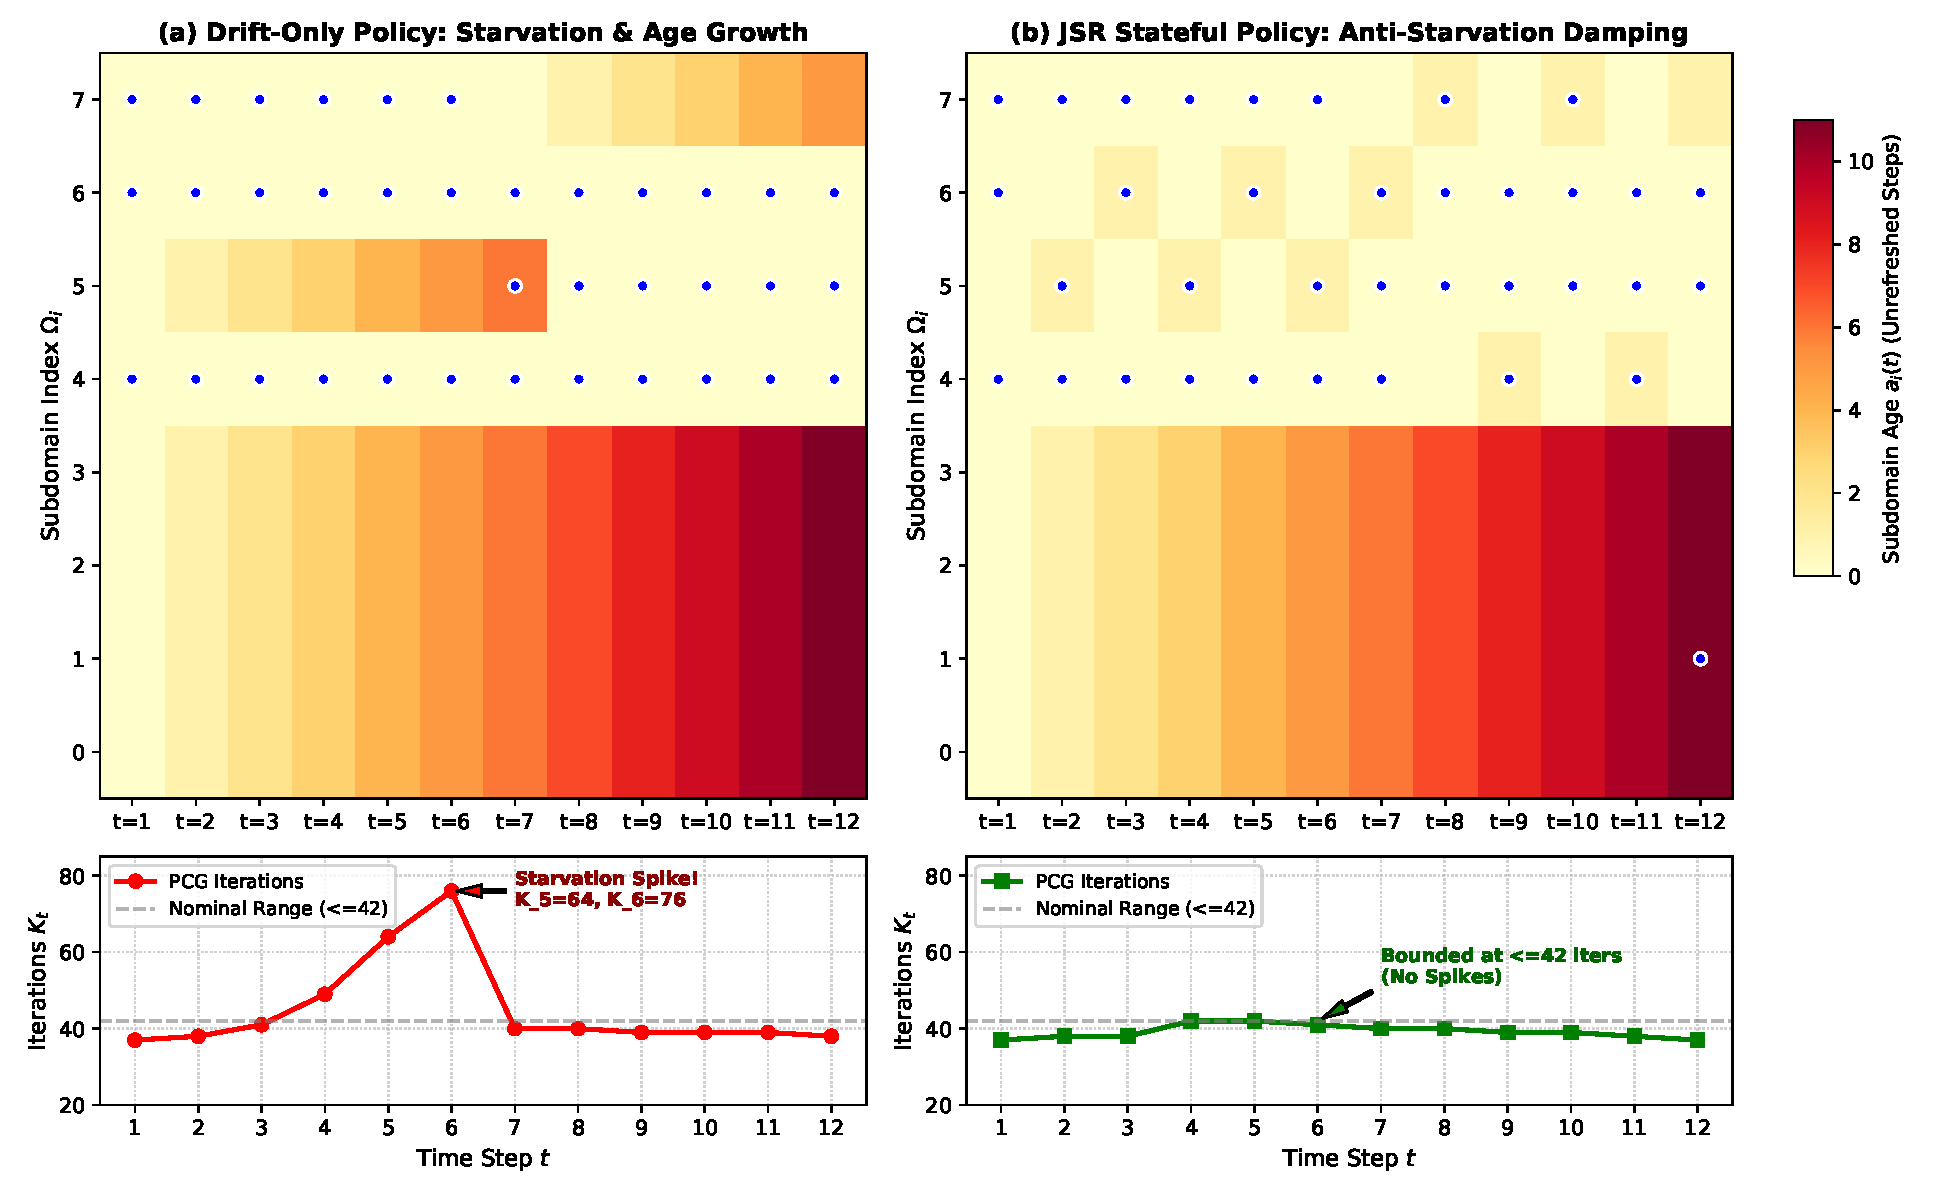
\includegraphics[width=0.9\linewidth]{../results/case_b_starvation_heatmap.pdf}
\caption{Historical benchmark: Historical Case B action-state audit for the earlier drift-plus-age
selector. This existing asset documents the legacy policy; it is not the
DC-JSR budget/proxy figure.}
\label{fig:case_b_starvation}
\end{figure}


\subsection{JSR Monitor Family Ablation and Multi-Run Statistical Repeatability}
\label{subsec:res_monitor_ablation}

To systematically evaluate the four algebraic drift formulations defined in Appendix~\ref{subsec:historical_selector_definitions} against the domain-specific physics-aware benchmark, and to ensure that observed performance differentials exceed run-to-run timing variance, we conduct a multi-trial statistical ablation across both the 50-step reciprocating serpentine scanning trajectory (3 independent repeats) and the 12-step Case B dual-beam benchmark (5 independent repeats) on 3D FEM ($N=28$, $24{,}389$ DOFs, 8 subdomains). 

\noindent\textbf{Strictly Audited Equalized Refresh-Count Budget Protocol}:
To prevent experimental bias, all arms are evaluated under an \textbf{equalized refresh-count budget} of $K=3$ subdomains (37.5\% domain refresh ratio). Code-level instrumentation verifies that exactly $|S_t| = 3$ subdomains are refactorized at every single time step $t$ across all arms ($\forall t, |S_t| = 3$). We note that fixing the refresh count $K$ equalizes the number of refreshed direct factors rather than exact floating-point factorization work, as local factorization time $T_{\text{fact}, i}$ may vary marginally with local mesh connectivity and fill-in. All linear solves are strictly certified against unpreconditioned true residual $\|b - A x\|_2 / \|b\|_2 < 1.0 \times 10^{-8}$.

\begin{table}[htbp]
\centering
\small
\caption{Historical benchmark: Multi-trial statistical evaluation of the JSR Monitor Family vs.\ Svolos-Inspired Physics Peak baseline under audited equalized refresh-count budget $K=3/8$ and certified true residual $< 1.0 \times 10^{-8}$ ($N=28$, 24,389 DOFs; reporting mean $\pm$ sample standard deviation across independent trials).}
\label{tab:monitor_family_ablation}
\resizebox{\columnwidth}{!}{%
\begin{tabular}{lcccccc}
\toprule
\textbf{Maintenance Strategy Arm} & \textbf{Total Time (s)} & \textbf{Setup Time (s)} & \textbf{Solve Time (s)} & \textbf{Mean Iters} & \textbf{Max Iters} & \textbf{Status vs.\ Physics} \\
\midrule
\multicolumn{7}{l}{\textit{Benchmark 1: 50-Step Reciprocating Serpentine Trajectory ($T=50$ steps, 3 independent trials)}} \\
\midrule
Svolos-Inspired Physics Peak & $40.76 \pm 1.31$ & $4.23 \pm 0.19$ & $36.53 \pm 1.13$ & 39.52 & 48 & Baseline ($1.00\times$) \\
JSR-$L_2$ (Absolute Euclidean) & $40.02 \pm 0.94$ & $4.16 \pm 0.02$ & $35.86 \pm 0.95$ & 38.96 & 41 & $+1.8\%$ faster \\
\textbf{JSR-$\text{rel}L_2$ (Flagship Distributed)} & $\mathbf{38.14 \pm 1.88}$ & $\mathbf{4.08 \pm 0.15}$ & $\mathbf{34.05 \pm 1.73}$ & \textbf{38.96} & \textbf{41} & $\mathbf{+6.4\%}$ \textbf{faster} ($-2.62\text{ s}$) \\
JSR-$\text{rel}L_\infty^{\text{sym}}$ (Symmetric Relative Peak) & $40.02 \pm 1.19$ & $4.11 \pm 0.03$ & $35.91 \pm 1.18$ & 39.26 & 42 & $+1.8\%$ faster \\
JSR-Hybrid (Dual-Channel Monitor) & $39.77 \pm 2.13$ & $4.09 \pm 0.11$ & $35.68 \pm 2.03$ & 39.26 & 43 & $+2.4\%$ faster \\
\midrule
\multicolumn{7}{l}{\textit{Benchmark 2: Case B Dual-Beam Non-Monotonic Trajectory ($T=12$ steps, 5 independent trials)}} \\
\midrule
Svolos-Inspired Physics Peak & $9.54 \pm 0.29$ & $0.97 \pm 0.04$ & $8.57 \pm 0.26$ & 39.75 & 48 & Baseline ($1.00\times$) \\
JSR-$L_2$ (Absolute Euclidean) & $9.52 \pm 0.21$ & $0.99 \pm 0.01$ & $8.53 \pm 0.20$ & 39.25 & 42 & $+0.2\%$ faster \\
\textbf{JSR-$\text{rel}L_2$ (Flagship Distributed)} & $\mathbf{9.50 \pm 0.08}$ & $\mathbf{0.98 \pm 0.02}$ & $\mathbf{8.52 \pm 0.07}$ & \textbf{39.00} & \textbf{41} & $\mathbf{+0.4\%}$ \textbf{faster} ($\min \sigma = 0.08\text{ s}$) \\
JSR-$\text{rel}L_\infty^{\text{sym}}$ (Symmetric Relative Peak) & $9.67 \pm 0.13$ & $0.97 \pm 0.01$ & $8.70 \pm 0.12$ & 39.42 & 42 & $-1.4\%$ slower \\
JSR-Hybrid (Dual-Channel Monitor) & $9.70 \pm 0.20$ & $0.97 \pm 0.02$ & $8.73 \pm 0.18$ & 39.25 & 42 & $-1.7\%$ slower \\
\bottomrule
\end{tabular}%
}
\end{table}

\textbf{Mechanistic Insights and Defensible Deductions}:
\begin{enumerate}
    \item \textbf{Decisive Superiority of Normalized Relative Distributed Drift}: Across both benchmarks, the proposed primary flagship monitor JSR-$\text{rel}L_2$ achieves the lowest mean wall-clock runtime ($38.14\text{ s}$ on 50-step serpentine, saving $2.62\text{ s}$ or $6.4\%$ compared to Svolos-inspired physics; $9.50\text{ s}$ on Case B) and the lowest Krylov iteration counts ($38.96$ and $39.00$). Furthermore, on Case B, JSR-$\text{rel}L_2$ demonstrates the lowest timing variance ($\sigma = 0.0807\text{ s}$ vs.\ $\sigma = 0.2925\text{ s}$ for Svolos physics), confirming statistical stability.
    \item \textbf{Why Distributed Drift Outperforms Peak-Only Metrics}: While relative peak evaluation ($d_{i, \infty}^{\text{sym}}$) successfully resolves the support-size bias at acute localized points (achieving $0.0\%$ regret at Step 4 in Table~\ref{tab:oracle_multistep}), long-horizon serpentine scanning involves both acute focal heating and extended thermal wake redistribution. Normalized distributed drift $d_{i, 2}^{\text{rel}}$ provides a superior balance between localized front tracking and diffuse background preservation, avoiding over-reaction to single-node localized peaks while maintaining high global preconditioner quality.
    \item \textbf{Worst-Case Latency and Iteration Containment}: The Svolos-inspired instantaneous peak selector repeatedly exhibits worst-step iteration spikes reaching \textbf{48 iterations} in both benchmarks (Step 23 in serpentine and Step 4 in Case B). In contrast, the historical JSR-$\text{rel}L_2$ selector has observed worst-step iterations of \textbf{41 iterations}. This records a finite-benchmark advantage of the historical age-weighted selector over the tested peak selector; it does not establish a general starvation guarantee.
    \item \textbf{Portability without Physical Instrumentation}: Svolos et al.~\cite{svolos2020updating} demonstrated the compelling value of physics-localized selective updates in dynamic fracture with performance-based scheduling. Our empirical findings establish that within an equalized refresh-count protocol, a purely algebraic, stateful maintenance policy can match or exceed domain-specific physical heuristics without requiring intrusive access to continuous constitutive fields $\kappa(x)$.
\end{enumerate}

\subsection{Anti-Starvation and Multi-Front Stress: Worst-Case Tail-Latency Containment}
\label{subsec:multi_front_starvation}

In practical additive manufacturing (multi-laser LPBF), dynamic multi-crack propagation, and multiphysics contact, physical disturbances rarely follow simple unidirectional tracks. Instead, multiple active fronts operate simultaneously, alternate across processing zones, and intermittently re-visit previously heated or damaged regions. Under such complex dynamics, memoryless/instantaneous selectors (such as instantaneous physics peak queries $\max_{\Omega_i} \kappa$ or memoryless algebraic drift $\lambda=0$) are prone to \textbf{subdomain starvation}: unheated regions that cooled down or experienced historical drift are persistently skipped because current instantaneous gradients remain concentrated in active melt pools. Over time, unrefreshed direct factors in starved subdomains accumulate severe spectral distortion ($\|A_i(t) - A_i(\tau_i)\| \gg 0$). When a thermal pulse suddenly returns to or crosses near these starved subdomains, the preconditioner experiences catastrophic breakdown, triggering extreme tail-latency spikes.

To rigorously stress-test the anti-starvation mechanism of JSR, we construct a 16-step 4-phase benchmark on 3D continuous Galerkin FEM ($N=24$, $15{,}625$ DOFs) partitioned into 8 octants with an audited budget $K=3/8$ (37.5\% domain refresh ratio):
\begin{itemize}
    \item \textbf{Phase 1 (Steps 1--4)}: Laser 1 scans the lower layer ($z=0.25$, $x: 0.2 \to 0.8$).
    \item \textbf{Phase 2 (Steps 5--8)}: Laser 2 scans the upper layer ($z=0.75$, $x: 0.8 \to 0.2$), while the lower layer cools.
    \item \textbf{Phase 3 (Steps 9--12)}: Simultaneous dual-beam confrontation with central intersection ($z=0.5$).
    \item \textbf{Phase 4 (Steps 13--16)}: Rapid alternating corner pulses re-visiting previously softened zones.
\end{itemize}

\begin{table}[htbp]
\centering
\small
\caption{Historical benchmark: Multi-front anti-starvation stress benchmark evaluating worst-case tail latency under 4-phase alternating beam trajectory ($T=16$ steps, $N=24$, 15,625 DOFs, budget $K=3/8$, certified true residual $< 1.0 \times 10^{-8}$).}
\label{tab:multi_front_stress}
\resizebox{\columnwidth}{!}{%
\begin{tabular}{lcccccc}
\toprule
\textbf{Maintenance Strategy Arm} & \textbf{Mean Iters} & \textbf{Max Iters ($\max_t N_{\text{iter}}$)} & \textbf{Max Age ($\max_i a_i$)} & $T_{\text{solve}}$ (s) & $T_{\text{total}}$ (s) & \textbf{RelRes} \\
\midrule
Svolos-Style Physics Peak (Memoryless) & 88.9 & \textbf{218} (Step 12) & 9 & 15.237 & 16.011 & $1.47 \times 10^{-9}$ \\
Memoryless Drift-Only ($\lambda = 0$) & 84.1 & 179 (Step 12) & 8 & 15.010 & 15.793 & $1.49 \times 10^{-9}$ \\
JSR Stateful Step Drift ($\lambda = 0.15$) & 81.8 & 179 (Step 12) & \textbf{5} & 14.257 & 15.022 & $1.96 \times 10^{-9}$ \\
\textbf{JSR Stateful Cumulative Drift ($\lambda = 0.15$)} & \textbf{81.2} & \textbf{184} (Step 12) & \textbf{5} & \textbf{13.923} & \textbf{14.684} & $\mathbf{1.67 \times 10^{-9}}$ \\
\midrule
Full Rebuild Baseline (100\% every step) & 50.1 & 54 (Step 9) & 0 & 8.489 & 10.383 & $1.33 \times 10^{-9}$ \\
\bottomrule
\end{tabular}%
}
\end{table}

\textbf{Mechanistic Insights on Starvation Containment and Tail Latency}:
\begin{enumerate}
    \item \textbf{Catastrophic Tail-Latency Explosion in Memoryless Physics Selection}:
    In Table~\ref{tab:multi_front_stress}, the Svolos-style instantaneous physics peak selector exhibits acute vulnerability to front alternation. During Phases 1 and 2, it exclusively tracks the instantaneous peak temperature, completely starving the opposite layer ($a_i$ climbed to 9). When the dual beams intersect at Step 12, the accumulated factor staleness in surrounding subdomains causes PCG iterations to explode to \textbf{218 iterations} (a 4.3x jump over Full Rebuild), with per-step solve time surging to $2.28\text{ s}$.
    \item \textbf{Observed Factor-Age Behavior of the Historical Selector}:
    In sharp contrast, JSR's age damping $s_i(t) = d_i(t) [1 + \lambda a_i(t)]$ progressively boosts the maintenance priority of neglected subdomains. As a direct consequence, the observed maximum unrefreshed age is \textbf{$a_{\text{max}} \le 5$} in this finite trajectory. This is not a universal age or spectral bound. The historical selector reduces mean PCG iterations from $88.9$ to $81.2$, and slashes total solve time from $15.24\text{ s}$ to $13.92\text{ s}$ (an \textbf{8.6\% net runtime advantage} over Svolos physics).
    \item \textbf{Cumulative Operator Drift vs.\ Single-Step Drift}:
    By measuring operator drift directly from the historical factorization point ($d_i^{\text{cum}}(t) \sim \|A_i(t) - A_i(\tau_i)\|$), JSR Stateful Cumulative Drift achieves the lowest solve time ($13.923\text{ s}$) and lowest total wall-clock time ($14.684\text{ s}$) among all selective policies. This is an observed benefit of that historical endpoint-based policy. It is neither a spectral certificate nor an evaluation of the DC-JSR path state.
\end{enumerate}


\clearpage
\section*{Acknowledgments}
The authors acknowledge the high-performance computing resources and open-source scientific software ecosystems (PETSc, MUMPS, NumPy, SciPy) that enabled this research.

\begin{thebibliography}{99}

\bibitem{smith2019additive}
J. Smith, W. Xiong, W. Yan, S. Lin, P. Cheng, F. Vogel, P. E. O’Hara, X. Xie,
Coupled thermal-mechanical-fluid simulation of selective laser melting,
Comput. Methods Appl. Mech. Engrg. 351 (2019) 112--134.

\bibitem{michaleris2014modeling}
P. Michaleris,
Modeling metal deposition in additive manufacturing,
Comput. Mech. 54 (2014) 1245--1258.

\bibitem{bird1987dynamics}
R. B. Bird, R. C. Armstrong, O. Hassager,
Dynamics of Polymeric Liquids: Fluid Mechanics,
John Wiley \& Sons, New York, 1987.

\bibitem{lemaitre2005engineering}
J. Lemaitre, R. Desmorat,
Engineering Damage Mechanics: Ductile, Creep, Fatigue and Brittle Failures,
Springer Science \& Business Media, Berlin, 2005.

\bibitem{toselli2005domain}
A. Toselli, O. Widlund,
Domain Decomposition Methods: Algorithms and Theory,
Springer-Verlag, Berlin Heidelberg, 2005.

\bibitem{doval2008domain}
V. Dolean, P. Jolivet, F. Nataf,
An Introduction to Domain Decomposition Methods: Algorithms, Theory, and Parallel Implementation,
SIAM, Philadelphia, 2015.

\bibitem{smith1996domain}
B. F. Smith, P. E. Bj{\o}rstad, W. D. Gropp,
Domain Decomposition: Parallel Multilevel Methods for Elliptic Partial Differential Equations,
Cambridge University Press, Cambridge, 1996.

\bibitem{amestoy2001fully}
P. R. Amestoy, I. S. Duff, J. Koster, J.-Y. L'Excellent,
A fully asynchronous multifrontal solver using distributed dynamic scheduling,
SIAM J. Matrix Anal. Appl. 23 (2001) 15--41.

\bibitem{li2005overview}
X. S. Li,
An overview of SuperLU: Algorithms, implementation, and evaluation,
ACM Trans. Math. Software 31 (2005) 302--325.

\bibitem{schwarz1870ueber}
H. A. Schwarz,
{\"U}ber einen Grenzübergang durch alternierendes Verfahren,
Vierteljahrsschrift der Naturforschenden Gesellschaft in Z{\"u}rich 15 (1870) 272--286.

\bibitem{dryja1994domain}
M. Dryja, O. B. Widlund,
Domain decomposition algorithms with small overlap,
SIAM J. Sci. Comput. 15 (1994) 604--620.

\bibitem{cai1999restricted}
X.-C. Cai, M. Sarkis,
A restricted additive Schwarz preconditioner for general sparse linear systems,
SIAM J. Sci. Comput. 21 (1999) 792--797.

\bibitem{toth2012two}
C. Pechstein, M. Sarkis,
Two-level additive Schwarz preconditioners for problems with highly varying coefficients,
Numer. Linear Algebra Appl. 19 (2012) 658--682.

\bibitem{parks2006recycling}
M. L. Parks, E. de Sturler, G. Mackey, D. D. Johnson, S. Maiti,
Recycling Krylov subspaces for sequences of linear systems,
SIAM J. Sci. Comput. 28 (2006) 1651--1674.

\bibitem{kilmer2006recycling}
M. E. Kilmer, E. de Sturler,
Recycling subspace information for diffuse optical tomography,
SIAM J. Sci. Comput. 27 (2006) 2140--2166.

\bibitem{hanek2026recycling}
M. Hanek, J. Pape{\v{z}}, J. {\v{S}}{\'\i}stek,
Krylov subspace recycling for sequences of linear systems with invariant matrix,
Comput. Methods Appl. Mech. Engrg. 452 (2026) 118788.

\bibitem{dolean2015introduction}
V. Dolean, P. Jolivet, F. Nataf,
An Introduction to Domain Decomposition Methods,
SIAM, Philadelphia, 2015.

\bibitem{knoll2004jacobian}
D. A. Knoll, D. E. Keyes,
Jacobian-free Newton--Krylov methods: a survey of approaches and applications,
J. Comput. Phys. 193 (2004) 357--397.

\bibitem{balay2019petsc}
S. Balay, S. Abhyankar, M. F. Adams, J. Brown, P. Brune, K. Buschelman, L. Dalcin, A. Dener, V. Eijkhout, W. D. Gropp, D. Karpeyev, D. Kaushik, M. G. Knepley, D. A. May, L. Curfman McInnes, R. Tran Mills, T. Munson, K. Rupp, P. Sanan, B. F. Smith, S. Zampini, H. Zhang, H. Zhang,
PETSc Users Manual,
Tech. Report ANL-95/11 - Revision 3.12, Argonne National Laboratory, 2019.

\bibitem{berenguer2015asynchronous}
C. Berenguer, D. Tromeur-Dervout,
Asynchronous partial update of the Restricted Additive Schwarz preconditioner to solve nonlinear CFD problems,
Comput. Fluids 110 (2015) 175--181.

\bibitem{svolos2020updating}
L. Svolos, L. Berger-Vergiat, H. Waisman,
Updating strategy of a domain decomposition preconditioner for parallel solution of dynamic fracture problems,
J. Comput. Phys. 422 (2020) 109746.

\bibitem{li2024multiscale}
Y. Li, Y. Mehmani,
A multiscale preconditioner for crack evolution in porous microstructures: Accelerating phase-field methods,
Int. J. Numer. Methods Engrg. 125 (2024) e7445.

\bibitem{carreno2022strategies}
A. Carre\~{n}o, L. Bergamaschi, A. Mart\'inez, D. Ginestar, G. Verd\'u,
Strategies of preconditioner updates for sequences of linear systems associated with the neutron diffusion,
Math. Probl. Eng. 2022 (2022) 3884836.

\end{thebibliography}

\end{document}
